\documentclass{report}
\title{Thesis proposal: Short-Term Outdoor Photometric Stereo}
\author{Yannick Hold-Geoffroy}
%\programme{Doctorat en g\'enie \'electrique}
%\annee{2015}


\date{\today}

%\usepackage{hyperref}
%\hypersetup{colorlinks,allcolors=ULlinkcolor}

%\frenchbsetup{%
%  CompactItemize=false,         % ne pas compacter les listes
%  ThinSpaceInFrenchNumbers=true % espace fine dans les nombres
%}


\usepackage[letterpaper, margin=1in]{geometry}
\usepackage[utf8]{inputenc}
\usepackage{times}
\usepackage{amsmath}
\usepackage{amssymb}
%\bibliographystyle{unsrtnat}
\usepackage[numbers,sort&compress]{natbib}
%\usepackage[numbers]{natbib}
%\usepackage{cite}   % sort citation numbers automatically
\usepackage{notoccite}
\usepackage{url}
\usepackage{graphicx}
\usepackage{rotating}
\usepackage{gensymb}
\usepackage{xcolor}
%\usepackage{adjustbox}
%\usepackage{authblk}
% to control spacing in item lists
\usepackage{enumitem}
\usepackage[pagebackref=false,breaklinks=true,colorlinks,bookmarks=false]{hyperref}
\usepackage{defs}

\linespread{1.5}


\begin{document}

%\frontmatter                    % pages liminaires

\maketitle
%\pagetitreonlyone                     % production des pages de titre

\tableofcontents

% Commands
\newcommand{\boldomega}{\boldsymbol \omega} % bold omega
\newcommand{\boldmu}{\boldsymbol \mu} % bold omega
\newcommand{\bolddelta}{\boldsymbol \delta} % bold delta

\newcommand\norm[1]{\left\lVert#1\right\rVert}

\newcommand\todo[1]{\textcolor{red}{#1}}

\graphicspath{{figures/}}


\chapter*{Symbols and notations}

\begin{table}[htbp]\caption{Symbols and notations}
\centering % to have the caption near the table
\begin{tabular}{r c p{10cm} }

\hline & & \\
$\langle \cdot, \cdot \rangle$      & $=$ & Scalar (dot) product \\
$\mathbf{x}$                        & $=$ & Vector \\
$X$                                 & $=$ & Matrix \\
$\omega$                            & $=$ & Angle \\
\hline
\end{tabular}
\label{tab:TableOfNotationForMyResearch}
\end{table}


%%%%%%%%%%%%%%%%%%%%%%%%%%%%%%%%%%%%%%%%%%%%%%%%%%%%%%%%%%%%%%%%%%%%%%%%%%%%%%%%
\chapter{Introduction}

Real world scanning of outdoors structures gained a lot of interest recently. The emergence of cheap and easy-to-use 3D sensors brought its share of new applications, enabling the digitization of the world by the masses. Most of common everyday 3D scanning devices are captive of the indoors, though. There is yet to find a way to give everyone the chance to scan building-scale objects, bridging the gap between indoor and outdoor scanning.

This thesis proposes to do so simply by using cameras, and an existing reconstruction technique dubbed "Photometric Stereo" (PS). The idea is to point a camera towards a scene to be scanned, and to capture a time-lapse sequence over time. Variations in the illumination conditions can be used by PS to reconstruct the shape of the observed scene. PS has been known in computer vision for more than 35 years, and is still an active area of research.

\section{Photometric Stereo}
\label{sec:ps_ori}

The first definition of PS, made in 1979 by Woodham~\cite{Woodham1979}, made a lot of assumptions to simplify the problem to its essence, such as these ones:

\begin{itemize} \setlength\itemsep{-0.2em}
  \item The object surface reflectance must be
  \vspace{-0.65em}\begin{itemize} \setlength\itemsep{0.1em}
    \item Lambertian;
    \item constant;
  \end{itemize} \vspace{-0.4em}
  \item Lighting is known;
  \item Lighting is a distant point light source;
  \item Sensors are noiseless;
  \item All the images are aligned.
\end{itemize}

Following these assumptions, the Lambertian image formation model for a single pixel is defined as
\begin{equation}
b_t =  \rho \; \mathbf{l} \mathbf{n}_t \quad,
\end{equation}
where pixel $t$ will have an intensity $b_t$ when the corresponding surface patch normal $\mathbf{n}_t$ of albedo $\rho$ is lit by a point light source with an incident vector $\mathbf{l}$. For the sake of simplification, its albedo. Likewise, the incident lighting vector $\mathbf{l}$ is scaled by its intensity.

This means that the appearance of a pixel in an image, with the aforementioned assumptions, is dependent on 1) the normal and albedo of a visible surface patch, and 2) the incident angle and intensity of the light. Woodham realized that if a pixel appearance depends on the surface normal, it meant that this surface normal can be found from a known pixel appearance. This means that the shape of an object (through its surface normals) could be obtained by observing the pixels appearance. But there's a problem: a single pixel intensity cannot explain all three degrees of freedom of the normal to be reconstructed (scaled by its albedo), leading to an underconstrained problem.

To solve this issue, it is possible to take a sequence of images, all from the same viewpoint, but with different lighting conditions. The shading difference between the different lighting conditions can constrain the problem correctly. In the case of a sequence of images, we define $L$ as the stacked incident vectors of all the $m$ images in the sequence (labeled $\mathbf{l}_{1}, \mathbf{l}_{2}, \dots \mathbf{l}_{m}$):
\begin{equation}
L =
\begin{bmatrix}
    \mathbf{l}_{1} \\
    \mathbf{l}_{2} \\
    \vdots \\
    \mathbf{l}_{m}
\end{bmatrix}
\quad,
\end{equation}
which can be used to define the appearance of all pixels over all the images of the sequence, as such:
\begin{equation}
\label{eq:lamb_refl}
\mathbf{b} =  \rho \mathbf{L} \mathbf{n} \quad.
\end{equation}

Solving eq.~\eqref{eq:lamb_refl} for $\mathbf{n}$ gives the relation
\begin{equation}
\label{eq:original_form}
\rho \mathbf{n} =  \mathbf{L}^{-1} \mathbf{b} \quad,
\end{equation}
giving birth to the Photometric Stereo technique.

$\mathbf{n}$ provides the structure of the scene visible in the image sequence, giving a single normal for each pixel of the image. This output is called a normal map, because it maps a surface normal to each surface patch visible by a pixel. Integrating this normal map results in an height map (also called depth map), which represents the height of the surface at each sample point. To summarize, PS outputs a normal map, the gradient of the height map.

A concrete example of PS can be seen in fig.~\ref{fig:PS_example}, where a sequence of images and its lighting directions are set as inputs of eq.~\eqref{eq:original_form} to give a normal map in output and its integrated surface.

The great strength of this technique is its output density: 3D information will be generated for every pixel of one input image. This means that a sequence of 5 megapixels images, as can be found on many current off-the-shelf cameras and cellphones, will generate an output of 5 million 3D points using PS. This quantity of information is impressive given the cost of point and shoot cameras and the ubiquity of cellphones.

Even with all the assumption we made, one issue remains: the lighting directions over the sequence must not be coplanar. If they are coplanar, eq.~\ref{eq:original_form} will result in an underconstrained system, leaving an unknown degree of freedom. This led Woodham to believe that PS ``does not apply to outdoor images taken at different times during the same day [...] since the sun's path across the sky is planar''.

%\begin{equation}
%\mathbf{b} = \rho L(\mathbf{\boldomega}) \langle \boldomega, {\bf n} \rangle \,,
%\end{equation}

\begin{figure}
\begin{tabular}{cccccc|ccc}
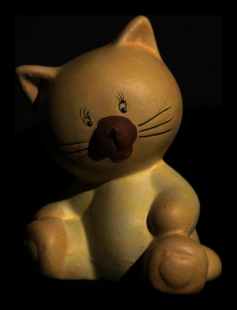
\includegraphics[width=.08\linewidth]{PS/cat_0.png} &
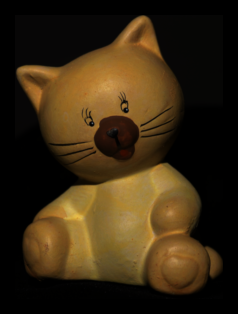
\includegraphics[width=.08\linewidth]{PS/cat_3.png} &
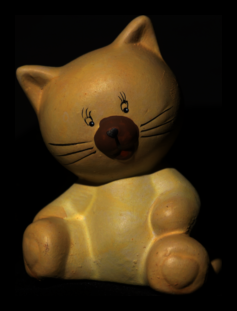
\includegraphics[width=.08\linewidth]{PS/cat_4.png} &
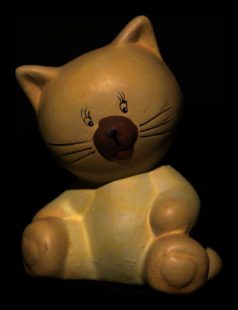
\includegraphics[width=.08\linewidth]{PS/cat_5.png} &
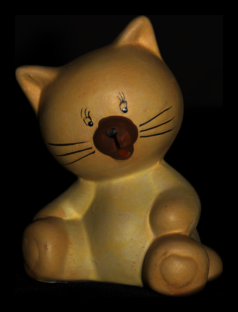
\includegraphics[width=.08\linewidth]{PS/cat_10.png} &
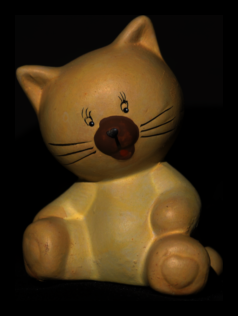
\includegraphics[width=.08\linewidth]{PS/cat_11.png} &

\includegraphics[width=.08\linewidth]{PS/cat_normal_map.png} &

\includegraphics[width=.04\linewidth]{PS/sphere_nm.png} &
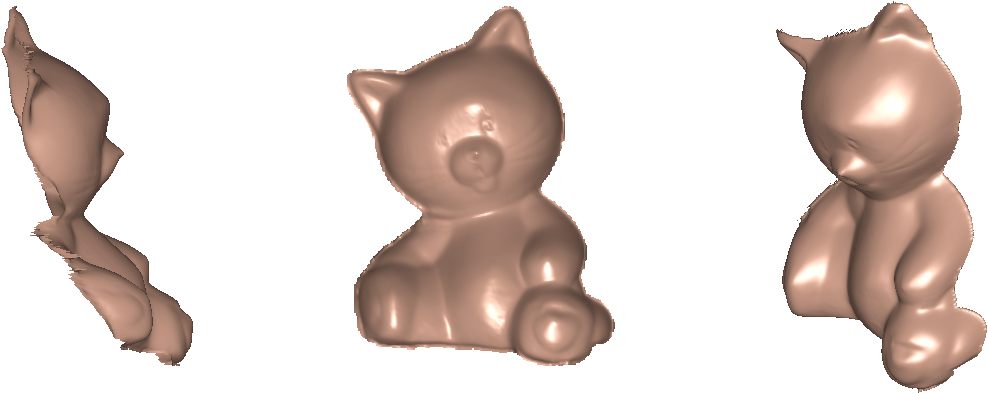
\includegraphics[width=.18\linewidth]{PS/3d.png} \\
a) & b) & c) & d) & e) & f) & g) & h) & i)
\end{tabular}
\caption{a-f) Examples of inputs lit from different directions, g) normal map obtained from the original form of the Photometric Stereo algorithm, h) sphere normal map showed as example, i) reconstructed surface from 3 viewpoints.\newline
{\small input images from CSE 455, 2010 by Neel Joshi, Ira Kemelmacher and Ian Simon}
}
\label{fig:PS_example}
\end{figure}

\section{Outdoor Photometric Stereo}

A lot of work have been done on PS since its original definition. Contrary to what Woodham believed, PS has recently been applied to outdoor photographs, mainly images captures by outdoor cameras. Unfortunately, outdoor lighting is complex and uncontrollable, therefore the techniques proposed in this domain require capturing either months of data, or the illumination conditions at each frame, none of which is a very practical scenario for the casual user.

To make PS work outdoor, the traditionally employed approximation models such as directional lighting will be replaced by a new data-driven model of natural illumination learned from a large database of high quality sky photographs. This database will be captured over extended periods of time, and will contain thousands of photos of the sky in different illumination conditions. By observing the sky directly, the data-driven model will accurately capture what the likely natural illumination conditions are for a given scene. This enhanced lighting model will better constrain the PS optimization algorithm, allowing it to converge toward real or plausible sky illumination conditions. The resulting shape estimation will better explain the observed input images, giving increased result quality. The key to bring PS outdoor is to understand natural illumination.

\section{Thesis proposal}

The main goal of this project is to reconstruct the shape of large-scale outdoor scenes from short time intervals, without the need for capturing the lighting conditions.

In this thesis, I propose to:
\begin{enumerate}
  \item bring a deeper understanding of the way PS can work outdoors;
  \item develop practical algorithms that allow precise shape recovery under unknown, uncontrolled outdoor lighting.
\end{enumerate}
These objectives can be attained by a better comprehension of natural illumination and its impact on shading. This knowledge can then be leveraged to improve existing reconstruction algorithms or make new ones that works with complex and uncontrolled lighting conditions.

This thesis will bring answers to questions like:
\begin{itemize}
  \item What is the minimum timelapse interval required to perform PS outside?
  \item What are the characteristics a PS practitioner needs to check in a sky to perform outside?
  \item How can we reconstruct an object with natural illumination using PS?
  \item What is the optimal input for PS when considering a 24h interval?
  \item Can we merge PS with other techniques to improve its performance outside?
\end{itemize}

\section{Anticipated impact}

3D scanning has become a part of everyday life, with sensors such as the Kinect now in everyone's home, effectively bringing 3D scanning capabilities to the masses. Taking the Kinect as example, a plethora of new use cases emerged since its original endeavor to revitalize the entertainment industry. For instance, the 3D printing market that grew significantly over the past few years, brought a new need for scans of household objects. Augmented reality is another avenue that requires a lot of models of real world objects. These are but a tiny fraction of the applications of real world scanning.

While the Kinect enabled myriads of applications in indoor environments, using such sensors outdoors is close to impossible. These kind of sensors are so-called active sensors, meaning that they interact with the scene to work. This usually means projecting light in the scene and sensing it back. But this method is problematic outside: the light patterns they emit are completely drowned by the sunlight. In outdoor settings, the only current possibility is to use very expensive scanners, out of reach for the casual user due to their complexity and operational cost. The idea is to bring back the availability and cheapness of sensors such as the Kinect to the outside world.

The level of understanding I propose in this thesis would allow the design and implementation a 3D shape acquisition system that relies only on off-the-shelf cameras, capable of bringing high quality digitization capabilities to anyone with a camera, thus enabling the collaborative reconstruction of large scale outdoor environments. This has the potential of impacting many fields, such as the digital preservation of cultural heritage before it gets damaged by wars, natural disasters, or the passage of time; the replication of real environments in virtual scenarios for the training of first responders or to improve urban planning; the creation of novel, realistic environments for use in video games or special effects in the movie industry; etc. By making these tasks easier, I believe this project will have significant impact on 3D shape acquisition as a whole.


%%%%%%%%%%%%%%%%%%%%%%%%%%%%%%%%%%%%%%%%%%%%%%%%%%%%%%%%%%%%%%%%%%%%%%%%%%%%%%%%
\chapter{State of the Art Review}
\label{c:sota}

% Expliquer les améliorations de la PS au travers du temps:
% \begin{itemize}
% 	\item Unknown lighting
% 	\item Unknown BRDF
% 	\item Robustness
% 	\item Outdoor (algorithme et analyse)
% 	\begin{itemize}
% 		\item Yu
% 		\item Boxin shi
% 	\end{itemize}
% \end{itemize}

Since its inception, Photometric Stereo has received a lot of attention throughout the years. Researchers tried to alleviate the restrictive assumptions of the original method, such as Lambertian reflectance, noiseless sensors and known lighting. This chapter will first relate briefly the major improvements made on PS over the years, and then focus on the efforts made to bring it outside the laboratory.


\section{Photometric Stereo}

As previously stated, PS has been studied extensively for many decades. Researchers worked to make the method more general by removing, or at least alleviating, the assumptions initially made.

\subsection{Surface reflectance}
% BRDF
One thing they did is make PS work on other surfaces than perfectly Lambertian ones. At first, specular reflections \cite{Ikeuchi1981} were studied and incorporated to the PS framework. This also brought the idea of distributed light sources instead of point light sources to the field, an important idea discussed later on. Over the years, most of the reflectance assumptions were removed, allowing PS to work on surfaces yielding varying reflectance using either a parametric~\cite{hertzmann-pami-05,goldman-tpami-10} or a data-driven approach~\cite{alldrin-cvpr-08}.

\subsection{Shape from Shading}
% SfS
A new technique called shape-from-shading~\cite{Horn1989} was born from Photometric stereo. In this technique, a bunch of priors is assumed to infer the structure from a single image instead of a sequence of images. Two interesting elements from this work are worth noting for general PS use: 1) the shadow detection and handling, and 2) uniform illumination (an ambient light source) is taken into account. This technique was further developed to take into account outdoor photometric cues on cloudy days~\cite{Langer1994}. This work recognized that cloudy days could be approximated as diffuse light sources and treated them differently than point light sources, a key insight that will be discussed in details in \ref{iccp15}. Lately, a framework to infer local shape based from shading cues was proposed~\cite{Xiong2013}, yielding interesting intuitions transferable to a PS algorithm. Even though work still continues on outdoors shape-from-shading~\cite{oxholm-eccv-12,johnson-cvpr-11,barron-pami-15}, it is of limited interest in the scope of this thesis. This is due to the fact that work on this technique has mainly focused on finding tight constraints, strong priors or semantic segmentation, which are interesting topics, but far from photometric and shading cues.

\subsection{Reconstruction algorithm improvements}
% Fusion with MVS
After the Shape from Shading spinoff, PS was also used in conjunction with other shape reconstruction techniques to enhance their performance. The main idea is to ally the strength of PS (usually its output density) with the strength of another technique. As an example, merging a Multi-View Stereo algorithm with PS was done with great success~\cite{HernandezEsteban2008}.
[Should I talk more about this?]

% Shadows and robustness
More recently, work has been done to increase the stability of and robustness to shadows, highlights, image noise~\cite{BarskyPetrou-pami-2003,ikehata-cvpr-12,ikehata-cvpr-14}.

\subsection{Lighting}
% Light sources arbitrary motion & Bas-Relief Ambiguity
The impact of illumination on PS has also been extensively studied. At first, still assuming point light sources, the case of unknown light directions was solved by using singular value decomposition along with a set of priors~\cite{Hayakawa1994}. This allowed to approximate the images lighting conditions and the surface normals jointly. It is worth of note that the reconstruction is always up to a bas-relief ambiguity in the case of unknown light sources~\cite{Belhumeur1999}. This means that every reconstruction with unknown light sources are up to a scaling factor that is impossible to determine theoretically.

% Optimal Illumination control
All this work suppose that the controlled light spans ``enough'' the space, meaning that the experimenter should stop when he feels he has enough data to work with. This brought the question: ``is there an optimal placement for the lights to optimize the reconstruction performance of PS?'' Many researchers thought that the optimal light placement was a tradeoff between ideal incident illumination and shadow coverage. Mathematically, having orthogonal light sources is optimal for the reconstruction, but where is it optimal? It was found that the optimal light position is a slant angle of 54.74\degree from the camera at equal distance in circles around it~\cite{spence-iwtas-03,drbohlav-iccv-05}. [figure]

% diffuse light
Contrarily to laboratory conditions, real world lighting is not purely directional. There is always an ambient illumination, also called uniform illumination. This ambient illumination is mainly due to reflections on surfaces like walls and floors and can be far from negligible when a strong light source such as the sun (through a window, for instance) is present. The impact of this ambient illumination on PS was recently looked into~\cite{Angelopoulou2013}. They show surprising results revealing that strong directional light is the most important factor to obtain good reconstruction performance. Useful results can be obtained even when the ambient illumination is up to nine times the strength of the directional lighting, as long as this directional lighting in itself is strong. Weak directional lighting produces bad results, even in the absence of ambient illumination.

% Arbitrary light sources
Research on indoors illumination made a big leap when generic lighting conditions were estimated alongside traditional PS~\cite{basri-ijcv-2007}. This work considered the illumination as a complete sphere around the scene instead of a sum of discrete point light sources. The lighting conditions recovered are, however, limited to low-frequencies. While it can be quite enough for simple materials, it won't work for materials exhibiting specularities or yielding non-Lambertian reflectance.

%Covering the vast amount of work done on PS as a whole is beyond the scope of this thesis proposal. The rest of the document will focus more closely on work that have considered PS on outdoor conditions.


\section{Outdoor Photometric Stereo}

% webcams
To tackle the new challenge that posed outdoor PS, a natural first strategy has been to experiment with Lambertian reflectance and to model the sun as a point light source, to match a well-studied lab condition. Unfortunately, approaches based on this model have practical limitations caused by the movement of the sun in the sky for a given day. Depending on the latitude and time of year, its trajectory may lie too close to a plane, yielding an under-constrained, two-source PS problem~\cite{hernandez-pami-11}. Possible solutions include waiting for a day when the sun trajectory is non-planar~\cite{shen-pg-14}, or capturing several months of data~\cite{ackermann-cvpr-12,abrams-eccv-12} to ensure good conditioning.

% single day
Recently, Shen~{\em et al.}~\cite{shen-pg-14} showed that, contrary to common belief, the sun path in the sky actually does not always lie within a perfect plane. Thus, PS reconstruction can sometimes be computed in a single day even with a point light source model. The main downside of this approach is that planarity of the sun path (\ie, conditioning of PS reconstruction) depends on the latitude and the time of year. More specifically, reconstruction becomes unstable at high latitudes near the winter solstice, and worldwide near the equinoxes.

% richer lighting models
To compensate for limited sun motion, a promising approach is to use richer models of illumination that account for additional atmospheric factors in the sky. Typically, more elaborate models of illumination is done by employing (hemi-)spherical high dynamic range (HDR) environment maps~\cite{debevec-siggraph-98,reinhard-book-05} as input to outdoor PS. Encouraging results have been reported in~\cite{yu-iccp-13} for outdoor images taken within an interval of just eight hours (in a single day). On one hand, full environment maps can be captured and used with calibrated PS algorithms~\cite{yu-iccp-13,shi-3dv-14,hung-wacv-15}. On the other hand, it is also possible to estimate part of the environment map without explicitly capturing it, by synthesizing a hemispherical model of the sky using physically-based models~\cite{inose-tcva-13,jung-cvpr-15}.

% hold-geoffroy
%The work presented below extends our initial analysis in~\cite{holdgeoffroy-iccp-15}. Rather than presenting a new reconstruction algorithm, in~\cite{holdgeoffroy-iccp-15} we conducted an empirical analysis of the same sky database to identify which days provide more favorable atmospheric conditions for outdoor PS. However, no consideration was given to the shortest time interval of data capture needed to obtain accurate reconstructions; all results were reported on at least 6 hours (a ``full day'') of captured data. Here, instead of comparing days, we focus on analyzing different time intervals within each day. We then show that 6 hours is actually more than necessary, and detail the relationship between the appearance of the sky hemisphere and the quality of PS reconstruction.


%%%%%%%%%%%%%%%%%%%%%%%%%%%%%%%%%%%%%%%%%%%%%%%%%%%%%%%%%%%%%%%%%%%%%%%%%%%%%%%%
\chapter{Existing contributions}
\label{ch:existing}

The work done so far on understanding outdoor illumination for use in PS is presented in this chapter. It mainly consist of data capture and its analysis.

First, the database of sky data is presented with its capture details and statistics. Then, our work on modeling the sky and its impact on one-day PS is presented~\cite{holdgeoffroy-iccp-15}. Lastly, our work on the link between what happens in the sky and the reconstruction performance is presented~\cite{holdgeoffroy-3dv-15}. The latter received an award for ``Best Paper (Runner Up)'' at 3DV 2015.

\section{HDR database}
\label{sec:hdrdb}

% From ICCP
%As one might expect, the answer to the question above is intrinsically tied to the orientation of a particular surface patch, the associated hemisphere of lighting directions observed by the patch, and the variation in lighting intensity in that hemisphere over the course of a day. So far, this question has only been explored in laboratory conditions or with simple directional illumination, where optimal lighting configurations can be theoretically derived~\cite{drbohlav-iccv-05,klaudiny-prl-14,shen-pg-14}. No attempt has been made at answering this question with more realistic illumination models in an outdoor setup, where lighting cannot be controlled and atmospheric effects are difficult to predict.

To analyze the influence of outdoor lighting on photometric stereo, we rely on a rich dataset of high dynamic range images of the sky, captured under a wide variety of conditions. We use the environment map database of \cite{lalonde-3dv-14}, which contains HDR images of the sky captured using the approach described in \cite{stumpfel-afrigraph-04}. We augment the dataset of~\cite{lalonde-3dv-14} with an additional set of images captured using a similar setup, but at a different geographical location. In all, the dataset we used for our analysis totals 3,800 illumination conditions, captured over 23 different days. To ensure the data is properly aligned temporally, the HDR sky photos were captured during a continuous 6 hour time interval on each of these days, from 10:30 until 16:30. Fig.~\ref{fig:database} shows examples of the sky environment maps used in our analysis. Note that while the examples have been tone mapped for display, the actual sky images have extremely high dynamic range, and span the full 22 stops required to properly capture outdoor lighting~\cite{stumpfel-afrigraph-04}. In addition, all the images are converted to grayscale before the analysis is performed.

% From JF's 3DV
%We introduce a novel dataset of image collections, where each image is associated with its ground truth HDR lighting conditions. In all, our dataset contains 1,850 images of 22 different outdoor landmarks, captured under 350 different illumination conditions, see fig. 2. Each image has high dynamic range, is radiometrically and geometrically calibrated, and is aligned with its corresponding light probe. In this section, we describe how the dataset was captured, calibrated and aligned. The dataset, software, and many additional results are available on the project website [1].

%In this work, we assume that outdoor scenes are illuminated by light emitted solely from the sun and sky, and ignore local illumination effects such as light bouncing off the ground or nearby objects. As such, we capture the outdoor lighting conditions with wide angle, HDR photographs of the entire sky hemisphere. To do so, we follow the approach proposed by Stumpfel et al. [22]. We captured seven exposures of the sky ranging from 1/8000 to 1 second, using a Canon EOS 5D Mark III camera installed on a tripod, and fitted with a SIGMA EXDG 8mm fisheye lens. A 3.0 ND filter was installed behind the lens, necessary to accurately measure the sun intensity. The exposures were stored as 14-bit RAW images at the full resolution of the camera. The camera was controlled using a Raspberry Pi via a USB connection, and the setup was mounted on the roof of a tall building to capture the entire sky hemisphere. The seven exposures were captured every two minutes over a span of between three and ten hours on 25 different days spread over a period of six months from June to December 2013. A total of 3,380 different lighting conditions were captured. The fisheye lens was radiometrically calibrated following [22] (to account for chromaticity shifts caused by the ND filter), geometrically calibrated using [19], and the resulting light probes mapped to the angular environment map representation [17] for storage in floating-point EXR format. We merged the seven exposures using [4] to create one HDR sky probe per exposure set. Because the camera may have shifted from one capture day to another, we automatically align all sky probes to the world reference frame.

%This was done by detecting the sun in at least 3 images for a given day, and by computing the rotation matrix which best aligned the detected positions and the real sun coordinates (obtained with [16]). For days when the sun was never visible, the probes were manually aligned using other aligned light probes as examples, and by matching visible buildings close to the horizon. The second row of fig. 2 shows examples sky probes captured with our system. Note that while the examples have been tone mapped for display, the actual sky probes have extremely high dynamic range (see fig. 3).

% Stats
~~~

\begin{figure*}[!th]
    \centering
    \setlength{\tabcolsep}{0pt}
	\newcommand{\customwidth}{.08\linewidth}
    \begin{tabular}{@{}rcccccccccccc@{}}
                                                     &
    \begin{minipage}{\customwidth}\centering\scriptsize 11:00 \end{minipage} &
    \begin{minipage}{\customwidth}\centering\scriptsize 11:30 \end{minipage} &
    \begin{minipage}{\customwidth}\centering\scriptsize 12:00 \end{minipage} &
    \begin{minipage}{\customwidth}\centering\scriptsize 12:30 \end{minipage} &
    \begin{minipage}{\customwidth}\centering\scriptsize 13:00 \end{minipage} &
    \begin{minipage}{\customwidth}\centering\scriptsize 13:30 \end{minipage} &
    \begin{minipage}{\customwidth}\centering\scriptsize 14:00 \end{minipage} &
    \begin{minipage}{\customwidth}\centering\scriptsize 14:30 \end{minipage} &
    \begin{minipage}{\customwidth}\centering\scriptsize 15:00 \end{minipage} &
    \begin{minipage}{\customwidth}\centering\scriptsize 15:30 \end{minipage} &
    \begin{minipage}{\customwidth}\centering\scriptsize 16:00 \end{minipage} &
    \begin{minipage}{\customwidth}\centering\scriptsize 16:30 \end{minipage}
    \\
    \begin{sideways}\begin{minipage}{\customwidth}\centering \scriptsize 08/24/2013 \\ light clouds \vspace{5pt} \end{minipage}\end{sideways} &
    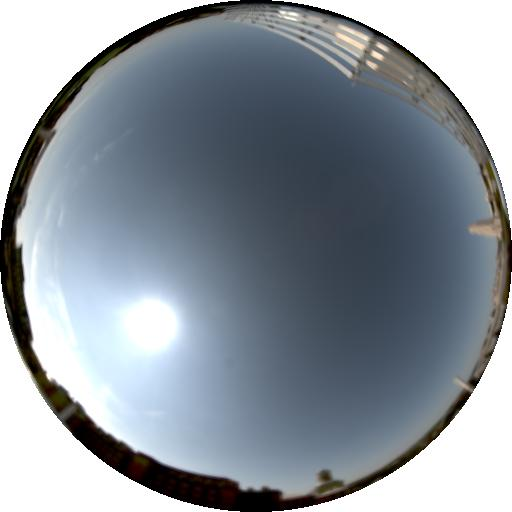
\includegraphics[width=\customwidth]{./figures/database/20130824_110040.jpg} &
    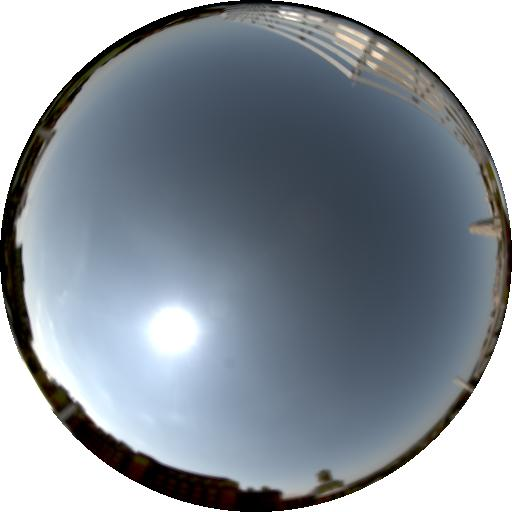
\includegraphics[width=\customwidth]{./figures/database/20130824_113038.jpg} &
    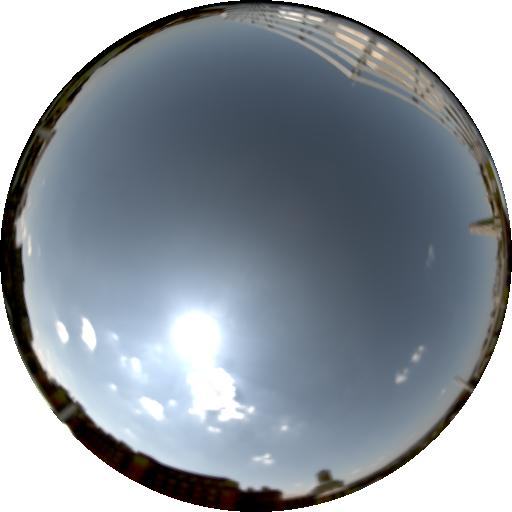
\includegraphics[width=\customwidth]{./figures/database/20130824_120033.jpg} &
    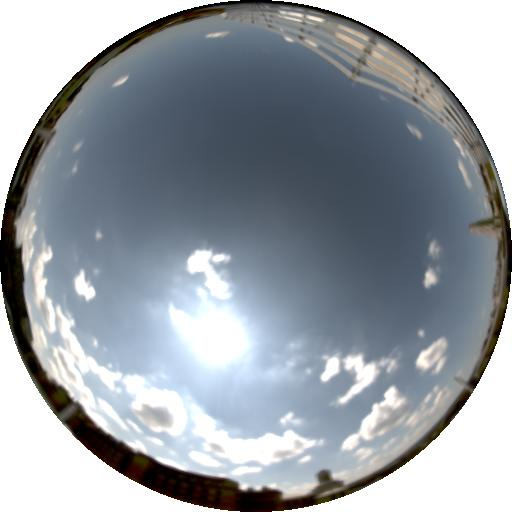
\includegraphics[width=\customwidth]{./figures/database/20130824_123024.jpg} &
    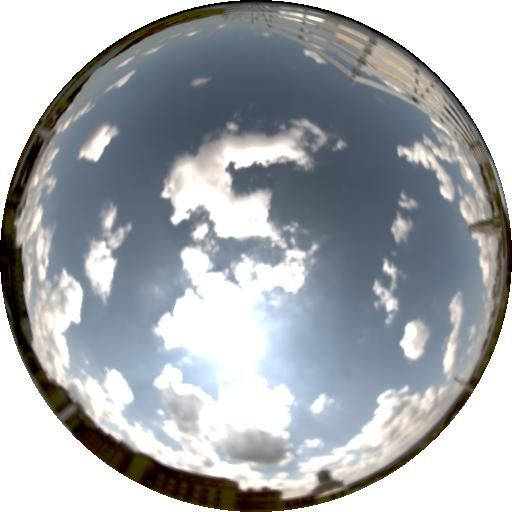
\includegraphics[width=\customwidth]{./figures/database/20130824_130014.jpg} &
    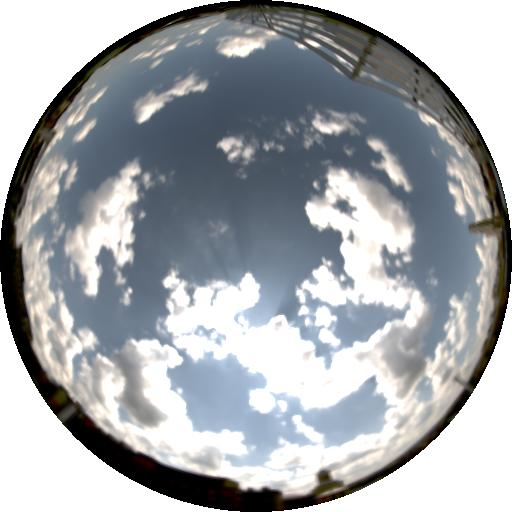
\includegraphics[width=\customwidth]{./figures/database/20130824_133006.jpg} &
    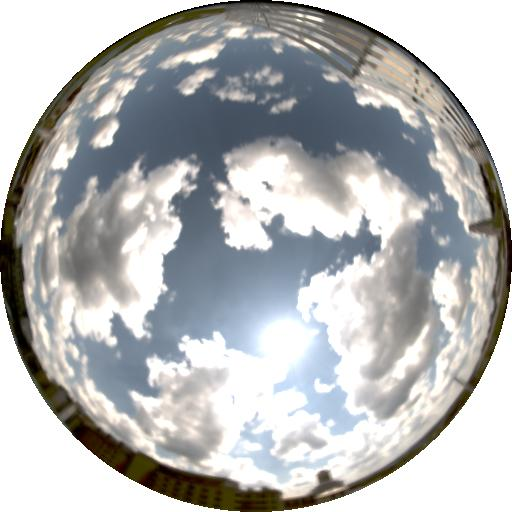
\includegraphics[width=\customwidth]{./figures/database/20130824_140002.jpg} &
    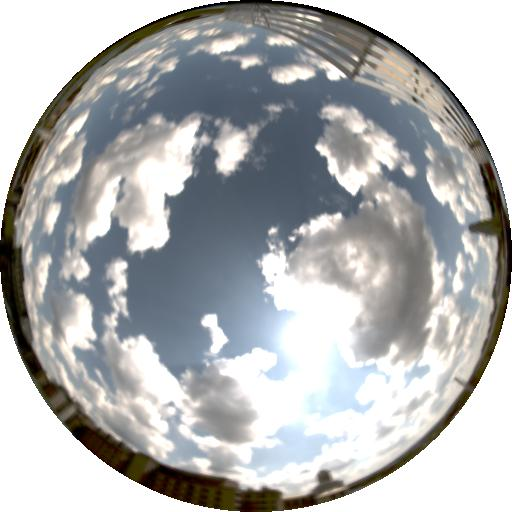
\includegraphics[width=\customwidth]{./figures/database/20130824_142960.jpg} &
    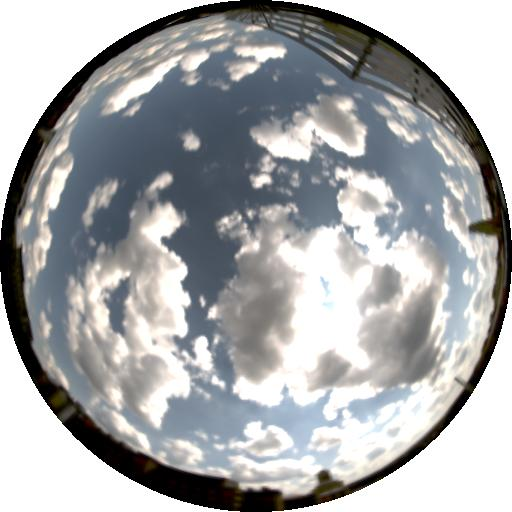
\includegraphics[width=\customwidth]{./figures/database/20130824_145957.jpg} &
    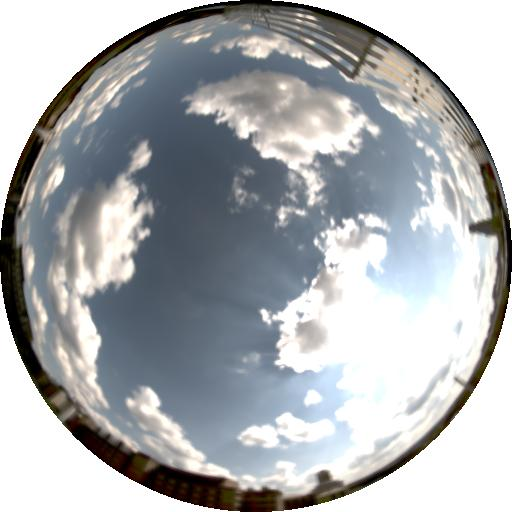
\includegraphics[width=\customwidth]{./figures/database/20130824_152946.jpg} &
    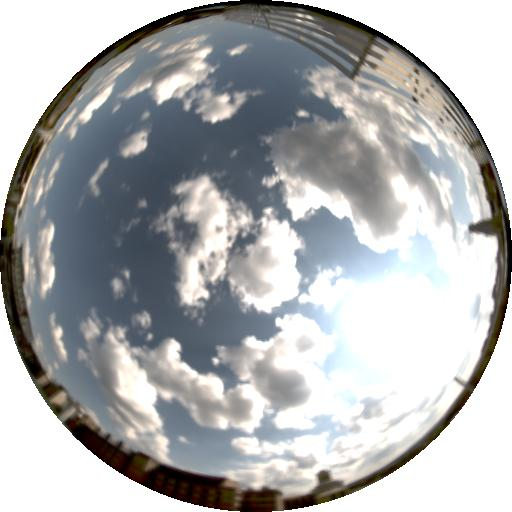
\includegraphics[width=\customwidth]{./figures/database/20130824_155938.jpg} &
    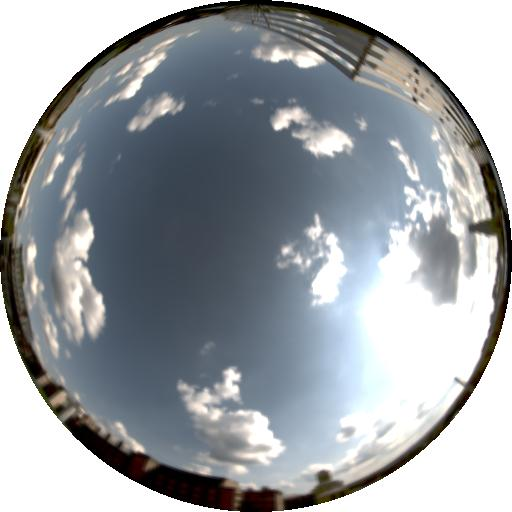
\includegraphics[width=\customwidth]{./figures/database/20130824_162933.jpg}
    \\
    \begin{sideways}\begin{minipage}{\customwidth}\centering \scriptsize 11/06/2013 \\ mixed \vspace{5pt} \end{minipage}\end{sideways} &
    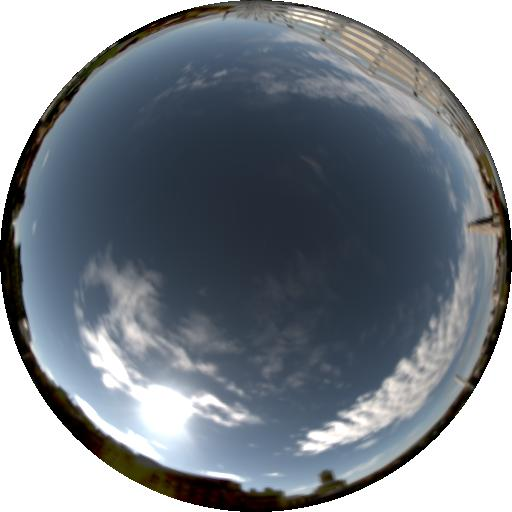
\includegraphics[width=\customwidth]{./figures/database/20131106_110951.jpg} &
    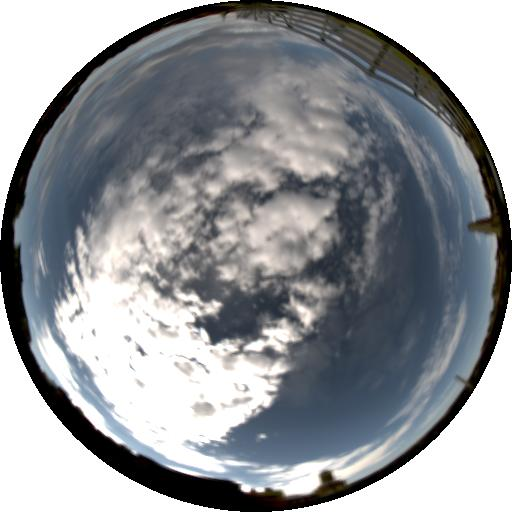
\includegraphics[width=\customwidth]{./figures/database/20131106_112948.jpg} &
    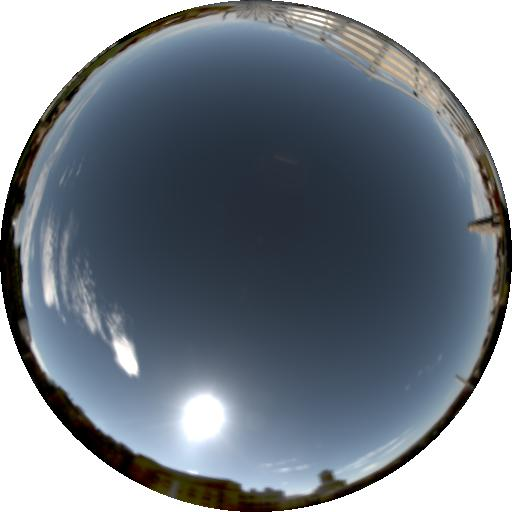
\includegraphics[width=\customwidth]{./figures/database/20131106_115943.jpg} &
    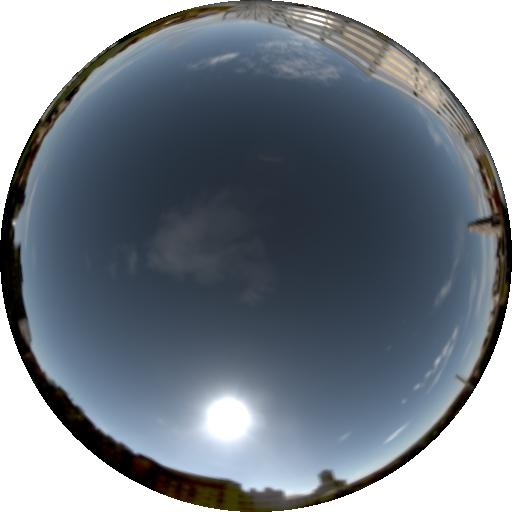
\includegraphics[width=\customwidth]{./figures/database/20131106_122939.jpg} &
    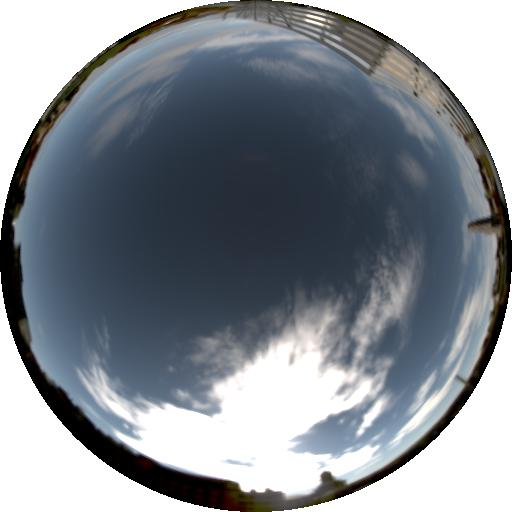
\includegraphics[width=\customwidth]{./figures/database/20131106_125937.jpg} &
    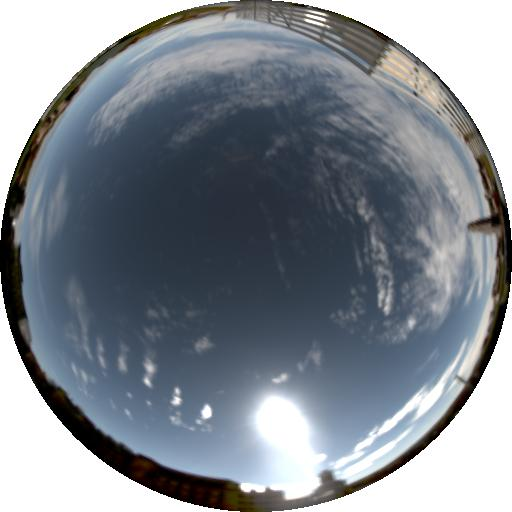
\includegraphics[width=\customwidth]{./figures/database/20131106_132936.jpg} &
    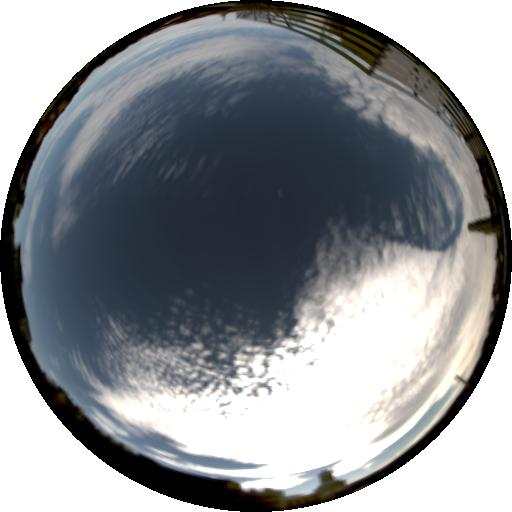
\includegraphics[width=\customwidth]{./figures/database/20131106_135932.jpg} &
    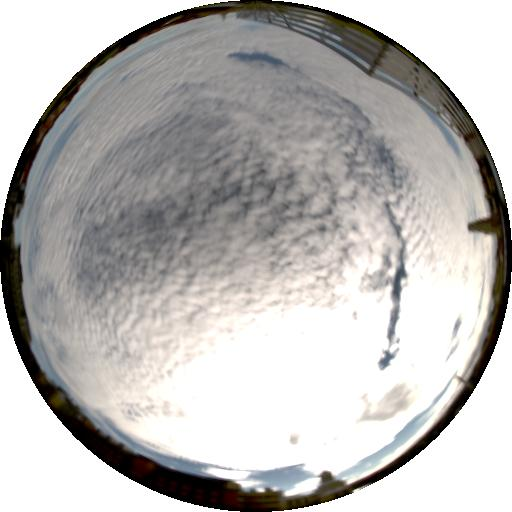
\includegraphics[width=\customwidth]{./figures/database/20131106_142922.jpg} &
    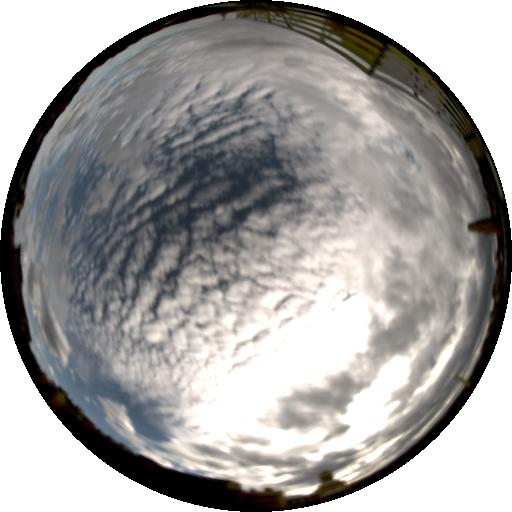
\includegraphics[width=\customwidth]{./figures/database/20131106_145915.jpg} &
    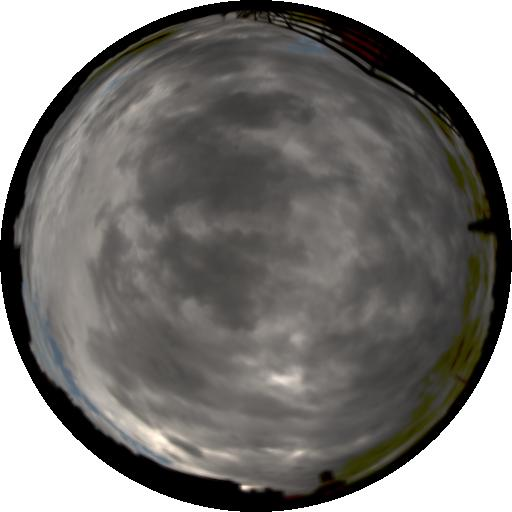
\includegraphics[width=\customwidth]{./figures/database/20131106_152913.jpg} &
    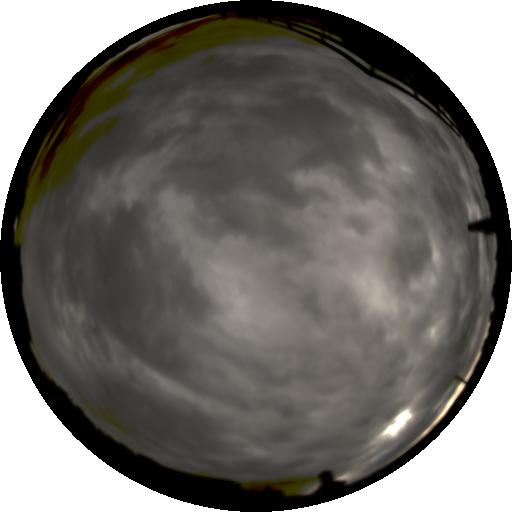
\includegraphics[width=\customwidth]{./figures/database/20131106_155906.jpg} &
    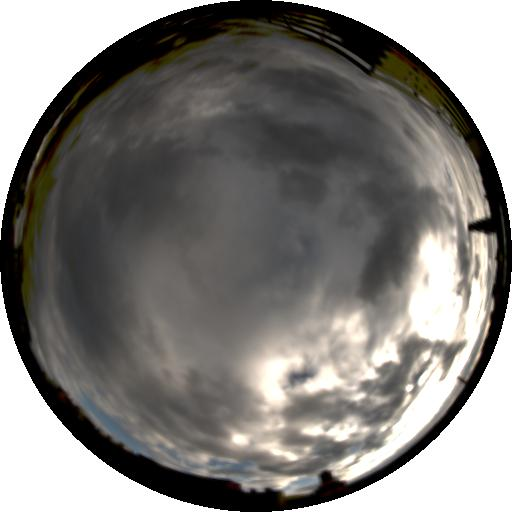
\includegraphics[width=\customwidth]{./figures/database/20131106_163057.jpg}

    \\
    \begin{sideways}\begin{minipage}{\customwidth}\centering \scriptsize 11/08/2014 \\ heavy clouds \vspace{5pt} \end{minipage}\end{sideways} &
    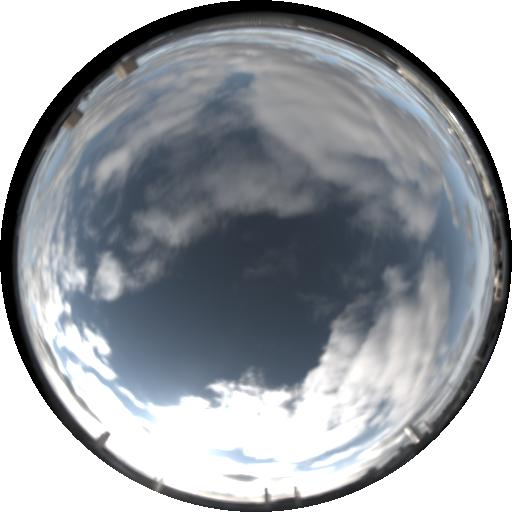
\includegraphics[width=\customwidth]{./figures/database/20141108_110025.jpg} &
    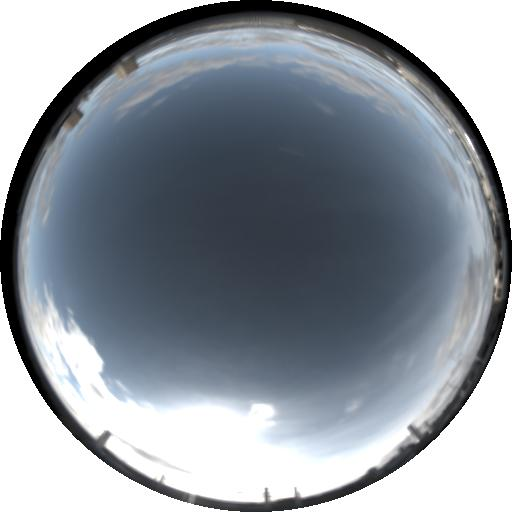
\includegraphics[width=\customwidth]{./figures/database/20141108_113025.jpg} &
    
\includegraphics[width=\customwidth]{./figures/database/20141108_120025.jpg} &
    
\includegraphics[width=\customwidth]{./figures/database/20141108_123025.jpg} &
    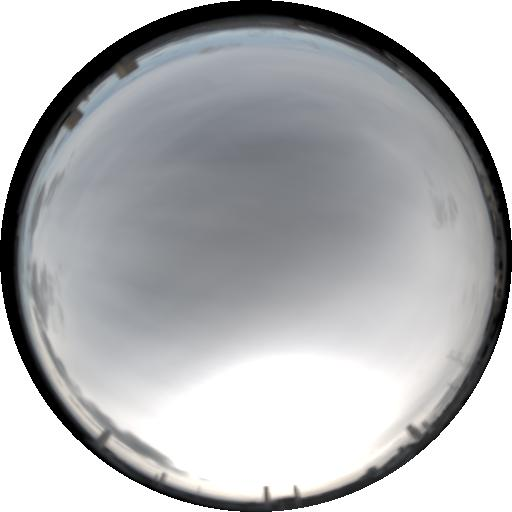
\includegraphics[width=\customwidth]{./figures/database/20141108_130025.jpg} &
    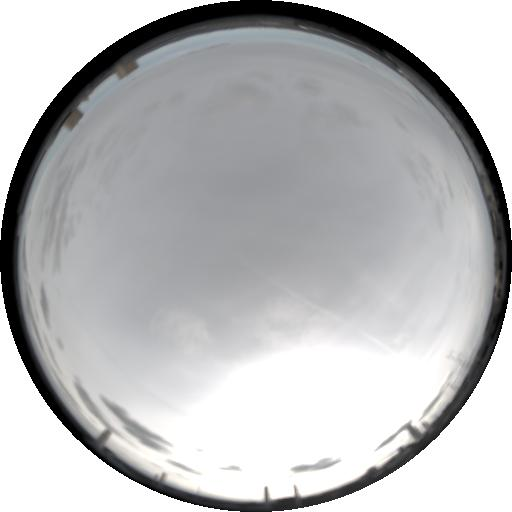
\includegraphics[width=\customwidth]{./figures/database/20141108_133025.jpg} &
    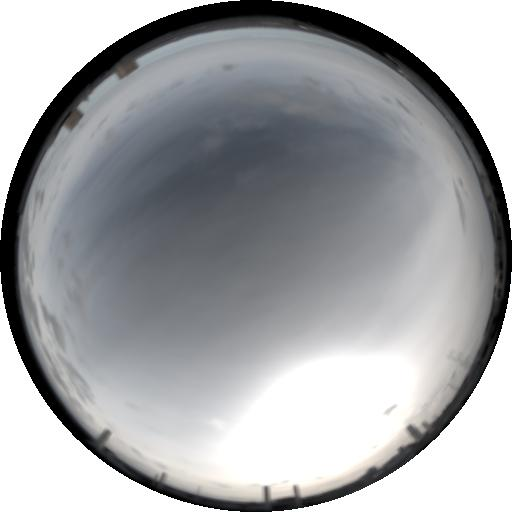
\includegraphics[width=\customwidth]{./figures/database/20141108_140025.jpg} &
    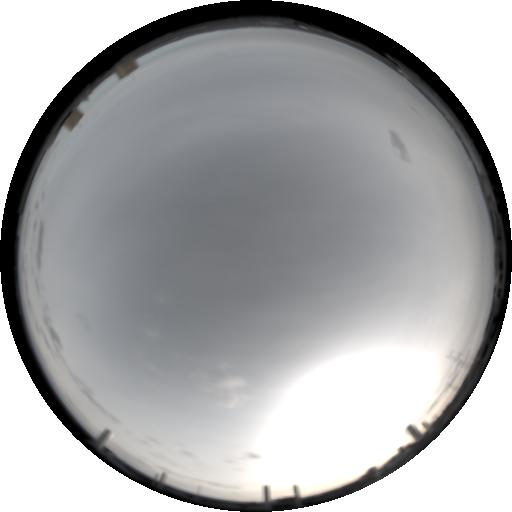
\includegraphics[width=\customwidth]{./figures/database/20141108_143025.jpg} &
    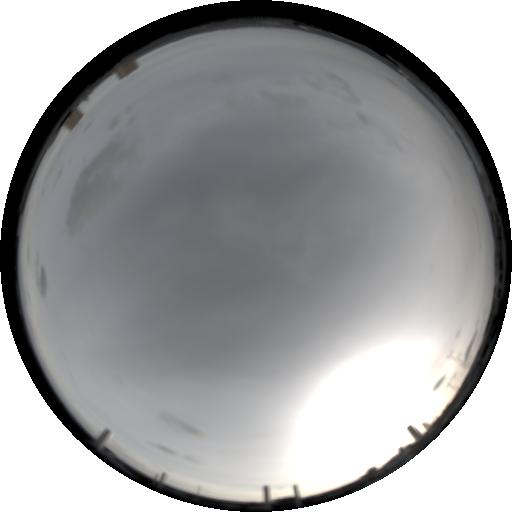
\includegraphics[width=\customwidth]{./figures/database/20141108_150025.jpg} &
    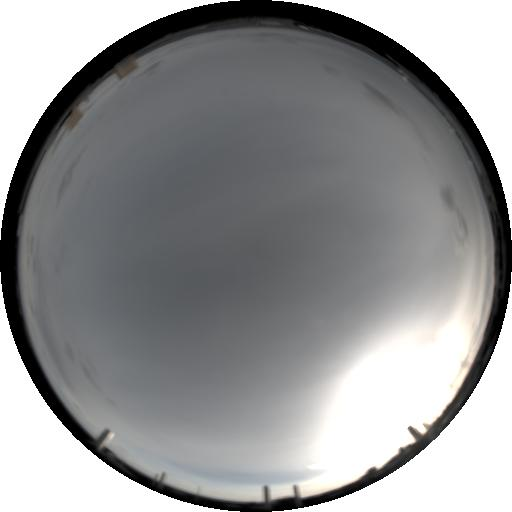
\includegraphics[width=\customwidth]{./figures/database/20141108_153025.jpg} &
    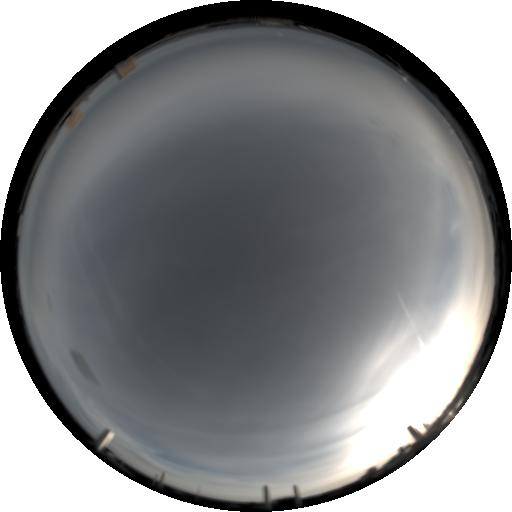
\includegraphics[width=\customwidth]{./figures/database/20141108_160025.jpg} &
    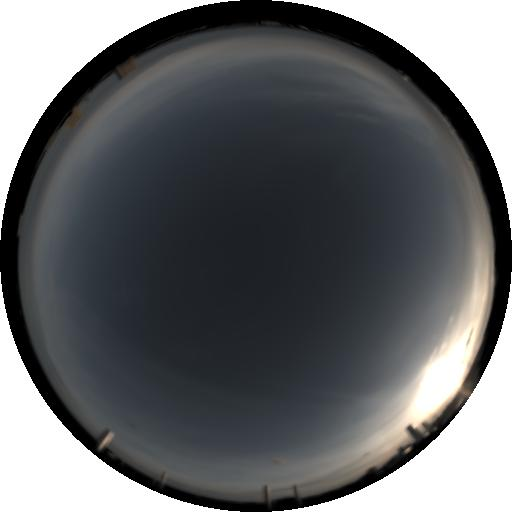
\includegraphics[width=\customwidth]{./figures/database/20141108_163025.jpg}

    \\

    \end{tabular}
   	\caption[]{Examples from our dataset of HDR outdoor illumination conditions. In all, our dataset contains 3,800 different illumination conditions, captured from 10:30 until 16:30, during 23 days, spread over ten months and at two geographical locations. Each image is stored in the 32-bit floating point EXR format, and shown tone mapped here for display (with $\gamma = 1.6$). The companion video\footnotemark shows time-lapse sequences for these sky environment maps.}
	\label{fig:database}
\end{figure*}

\section{What Is a Good Day for Outdoor Photometric Stereo?}
\label{iccp15}

%% !TEX root = main.tex

In this paper, we present a systematic analysis of the expected performance of photometric stereo algorithms in outdoor settings. To explore the influence of these effects, we exploit a large database of outdoor HDR environment maps, which provides a rich sampling of the variability in outdoor illumination. Through a theoretical analysis (inspired by \cite{sun-ivc-07}) and supported by an extensive empirical evaluation as well as a preliminary quantitative validation, we derive confidence intervals that allow us to predict when surface normals can be reconstructed more accurately and solely from the photometric cue. Instead of focusing exclusively on sun position~\cite{shen-pg-14}, our analysis incorporates the influence of all components of natural lighting: sun, sky, clouds, etc., as well as noise and surface albedo.

This paper does \emph{not} introduce a novel photometric stereo algorithm. Rather, we explore the conditions in which PS may or may not work, when faced with the challenging case of uncontrollable outdoor illumination. Our main goal is to provide guidance for future research by assessing the \emph{reconstructibility} of surface patches as a function of their orientation and the illumination conditions, given a set of HDR environment maps captured throughout a single day.

In this paper, we present a systematic analysis of the expected performance of photometric stereo algorithms in outdoor settings. To explore the influence of these effects, we exploit a large database of outdoor HDR environment maps, which provides a rich sampling of the variability in outdoor illumination. Through a theoretical analysis (inspired by \cite{sun-ivc-07}) and supported by an extensive empirical evaluation as well as a preliminary quantitative validation, we derive confidence intervals that allow us to predict when surface normals can be reconstructed more accurately and solely from the photometric cue. Instead of focusing exclusively on sun position~\cite{shen-pg-14}, our analysis incorporates the influence of all components of natural lighting: sun, sky, clouds, etc., as well as noise and surface albedo.

A promising approach to answer this question is to use more elaborate models of illumination---high dynamic range (HDR) environment maps~\cite{reinhard-book-05}---as input to outdoor PS. Promising results have been reported in~\cite{yu-iccp-13} for outdoor images taken within an interval of just eight hours (in a single day). However, the quality of outdoor results is reported to be inferior to that obtained in indoor environments, the decline being attributed to modest variation in sunlight. This observation leads to an interesting, yet unanswered question: had the sun path and atmosphere conditions been different on that day, could the quality of their results have been better? Or, in other words: what makes it a good day for outdoor Photometric Stereo?

As one might expect, the answer to the question above is intrinsically tied to the orientation of a particular surface patch, the associated hemisphere of lighting directions observed by the patch, and the variation in lighting intensity in that hemisphere over the course of a day. So far, this question has only been explored in laboratory conditions or with simple directional illumination, where optimal lighting configurations can be theoretically derived~\cite{drbohlav-iccv-05,klaudiny-prl-14,shen-pg-14}. No attempt has been made at answering this question with more realistic illumination models in an outdoor setup, where lighting cannot be controlled and atmospheric effects are difficult to predict.

In this paper, we present a systematic analysis of the expected performance of photometric stereo algorithms in outdoor settings. To explore the influence of these effects, we exploit a large database of outdoor HDR environment maps, which provides a rich sampling of the variability in outdoor illumination. Through a theoretical analysis (inspired by \cite{sun-ivc-07}) and supported by an extensive empirical evaluation as well as a preliminary quantitative validation, we derive confidence intervals that allow us to predict when surface normals can be reconstructed more accurately and solely from the photometric cue. Instead of focusing exclusively on sun position~\cite{shen-pg-14}, our analysis incorporates the influence of all components of natural lighting: sun, sky, clouds, etc., as well as noise and surface albedo.

This paper does \emph{not} introduce a novel photometric stereo algorithm. Rather, we explore the conditions in which PS may or may not work, when faced with the challenging case of uncontrollable outdoor illumination. Our main goal is to provide guidance for future research by assessing the \emph{reconstructibility} of surface patches as a function of their orientation and the illumination conditions, given a set of HDR environment maps captured throughout a single day.

% Assumptions
To make this novel analysis tractable, we make the following assumptions. We consider Lambertian surface patches, and assume that at most one day of data can be used. We also assume that the dominant part of the light comes from the sky hemisphere (sun, sky, clouds, etc.) and surface patches are independent (cast shadows and inter-reflections are not modeled).

Although previous work have presented sensitivity analyses for standard PS with point light sources (\eg,~\cite{sun-ivc-07,jiang-bunke-sp-91,klaudiny-prl-14,shen-pg-14}), so far as we know, the case of outdoor PS with more complex illumination models has received little attention.

\subsubsection{Image formation model}

Consider a small, Lambertian surface patch with normal vector ${\bf n}$ and albedo $\rho$ (w.l.o.g., assume albedo is monochromatic). At time $t$, this surface patch is observed under natural, outdoor illumination represented by the environment map $L_t(\boldomega)$ (\eg, fig.~\ref{fig:database}), with $\boldomega$ denoting a direction in the unit sphere. With an orthographic camera model, this patch is depicted as an image pixel with intensity
%
\begin{equation}
    b_t = \frac{\rho}{\pi} \int_{\Omega_{\bf n}} L_t(\mathbf{\boldomega}) \langle \boldomega, {\bf n} \rangle d\omega \,,
    \label{eqn:imageformation-continuous}
\end{equation}
%
where $\langle \cdot, \cdot \rangle$ denotes the dot product. Integration is carried out over the hemisphere of incoming light, $\Omega_{\bf n}$, defined by the local orientation ${\bf n}$ of the surface, fig.~\ref{fig:normal-diagram}. This hemisphere corresponds to an occlusion (or attached shadow) mask; only half of the pixels in the environment map contribute to the illumination of the surface patch. To make the analysis tractable and independent on object geometry, this paper focuses on the simpler case without cast shadows.

\begin{figure}
    \centering
    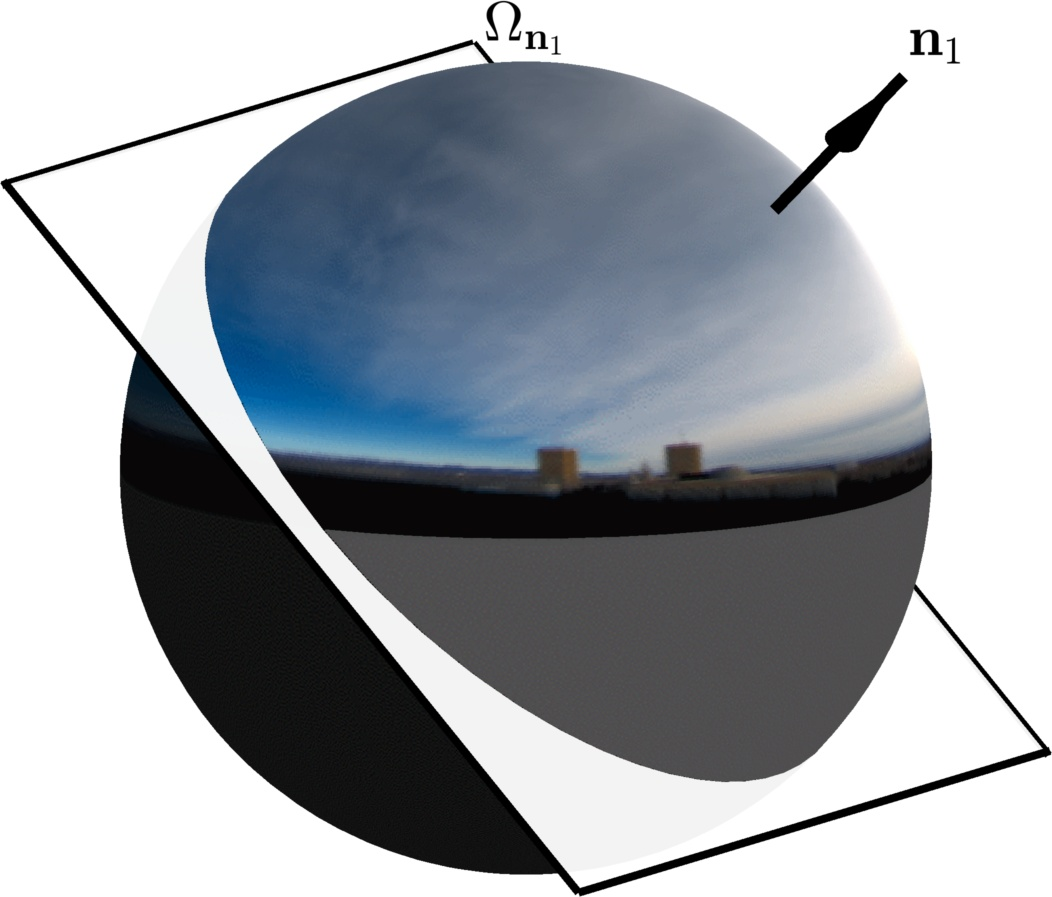
\includegraphics[width=.495\linewidth]{./figures/diagramFig/diagram1.jpg}
    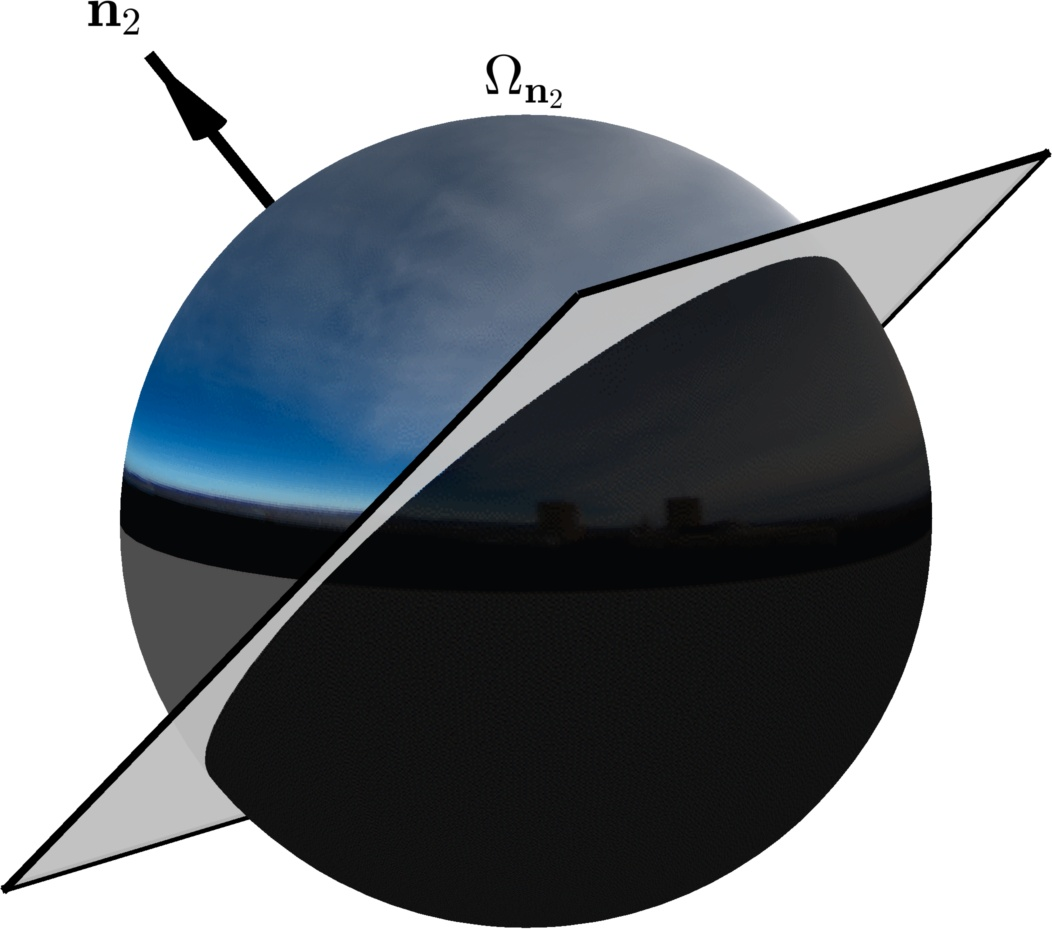
\includegraphics[width=.495\linewidth]{./figures/diagramFig/diagram2.jpg}
    \caption{A normal $\mathbf{n}$ defines an integration domain $\Omega_{\mathbf{n}}$ equivalent to a hemisphere on the entire spherical environment map. Only light emanating from this hemisphere contribute to the shading on that patch. Therefore, patches with different normals are lit differently even if the environment map is the same.}
    \label{fig:normal-diagram}
\end{figure}

This image formation model is then discretized as,
%
\begin{equation}
b_t = \frac{\rho}{\pi}\sum_{\boldomega_j \in \Omega_{\bf n}} \widehat{L}_t(\boldomega_j) \langle \boldomega_j, {\bf n} \rangle\,,
\label{eqn:imageformation-discrete}
\end{equation}
%
with $\widehat{L}_t(\boldomega_j) = L_t(\boldomega_j)\Delta\omega_j$ representing the environment map weighted by the solid angle $\Delta\omega_j$ spanned by pixel $j$ ($\Delta\omega_j$, $\forall j$, are normalized as to sum to $2\pi$). Eq.~$\eqref{eqn:imageformation-discrete}$ can be further summarized into the equivalent form
%
\begin{equation}
b_t = {\bf \bar l}_t^T \mathbf{x}
\label{eqn:imageformation-simplified}
\end{equation}
where ${\bf x} = \rho {\bf n}$ is the albedo-scaled normal vector and
\begin{equation}
{\bf \bar l}_t = \frac{1}{\pi} \sum_{\boldomega_j \in \Omega_{\bf n}} \widehat{L}_t(\boldomega_j) \boldomega_j \in \mathbb{R}^3
\label{eqn:mean-light}
\end{equation}
is interpreted as the {\em mean light vector} for the environment map at a time $t$.

Given multiple images taken at times $t \in \{1,2,\ldots,T\}$, we collect all photometric constraints for patch ${\bf x}$ to obtain:
\begin{equation}
\mathbf{b} =
\begin{bmatrix}
 b_1 \\ b_2 \\ \vdots \\ b_T
\end{bmatrix}
=
\begin{bmatrix}
 {\bf \bar l}_1^T \\ {\bf \bar l}_2^T \\ \vdots \\ {\bf \bar l}_T^T
\end{bmatrix}
{\bf x} = \mathbf{L} \mathbf{x} \,.
\label{eqn:matrix-form}
\end{equation}
With~\eqref{eqn:matrix-form}, this model of natural environmental illumination becomes quite similar to a model with a distant point light source, the well-known case in PS. However, note that each ${\bf \bar l}_t$ in ${\bf L}$ is a function of $\Omega_{\bf n}$ and, thus, of ${\bf n}$.

Most importantly, in outdoor PS, a well-defined solution ${\bf x}$ may exist even if the relative sun motion is nearly planar during a certain time interval. Instead of relying solely on sun direction, now, the solution requires non-coplanar mean light vectors ${\bf \bar l}_t$, which are determined by a comprehensive set of natural illumination factors.

\subsubsection{Modeling uncertainty}

From~\eqref{eqn:matrix-form}, the least-squares solution ${\bf x} = ({\bf L}^T{\bf L})^{-1}{\bf L}^T{\bf b}$ of outdoor PS is clearly affected by the condition number of ${\bf L}$. Thus, we next characterize how well the solution ${\bf x}$ is constrained by natural, outdoor illumination within a given time interval (\eg, one day)---which is encoded by the set of mean light vectors ${\bf \bar l}_t$ in ${\bf L}$ or, equivalently, the set of environment maps $L_t(\cdot)$.

To assess the reliability of a solution ${\bf x}$, we follow standard practice in PS~\cite{klaudiny-prl-14,sun-ivc-07} and consider image measurements corrupted by zero-mean Gaussian noise with equal variance $\sigma^2$ (as least squares estimation is only optimal for this practical, most common noise model). Thus, ${\bf b}$ in~\eqref{eqn:matrix-form} follows a normal distribution:
%
\begin{equation}
{\bf b} \sim \mathcal{N}\left( \boldmu_b, \sigma^2 {\bf I} \right)\,,
\end{equation}
%
where $\boldmu_b$ has the (unknown) uncorrupted pixel values.

Since the desired least-squares solution for the albedo-scaled normal, ${\bf x} = \left({\bf L}^T{\bf L}\right)^{-1}{\bf L}^T{\bf b}$, is a linear transformation of a Gaussian random vector, it is easy to show that
%
\begin{equation}
{\bf x} \sim \mathcal{N} \left( \boldmu_x, \sigma^2({\bf L}^T{\bf L})^{-1} \right)\,,
\end{equation}
where $\boldmu_x = \left({\bf L}^T{\bf L}\right)^{-1}{\bf L}^T\boldmu_b$ is the expected value of ${\bf x}$.
Once the albedo of a surface patch is known, we analyze its contribution to the uncertainty in the estimated normal vector, ${\bf n} = \rho^{-1}{\bf x}$, using a similar distribution,
%
\begin{equation}
{\bf n} \sim \mathcal{N} \left( \frac{\boldmu_x}{\rho}, \frac{\sigma^2}{\rho^2}({\bf L}^T{\bf L})^{-1} \right)\,.
\label{eqn:normal-distrib}
\end{equation}

The marginal distributions in~\eqref{eqn:normal-distrib} allow us to derive confidence intervals that indicate the uncertainty in each component of the least squares estimate ${\bf \hat n} = [ \hat n_x \ \hat n_y \ \hat n_z ]^T$ of ${\bf n} = [ n_x \ n_y \ n_z ]^T$. The corresponding $95\%$ confidence interval~\cite{hastie-book-09} is given by
%
\begin{equation}
\hat{\mathbf{n}} \pm \bolddelta \,, \quad \text{with } \delta_k = 1.96 \frac{\sigma\lambda_k}{\rho} \,,
\label{eqn:confidence-xyz}
\end{equation}
%
where $\lambda_k$ is the square root of the $k$th element on the diagonal of $({\bf L}^T{\bf L})^{-1}$. As expected, the sensor-dependent noise level $\sigma$ is not the only factor that determines uncertainty. The gain factor $\lambda_k/\rho$ in \eqref{eqn:confidence-xyz} reveals how outdoor illumination (the conditioning of ${\bf L}$) and albedo can amplify the effect of noise on the solution ${\bf \hat n}$. The lower the albedo $\rho$ is, the larger is the variance in the obtained estimate $\bf \hat n$ (as less light is reflected towards the camera). Our goal is then to answer the remaining question: how do natural changes in outdoor illumination affect this gain factor ($\lambda_k$) and, therefore, uncertainty?

\subsubsection{An intuitive measure of uncertainty}
\label{subsec:measure_uncertainty}

To provide a measure of uncertainty that is more intuitive than~\eqref{eqn:confidence-xyz}, we consider angular distances in degrees,
%
\begin{equation}
\theta^\pm = \cos^{-1}(\mathbf{n}^T{\bf \hat n}^\pm)\,,
\quad \text{where }
{\bf \hat n}^\pm = \frac{{\bf \hat n} \pm \bolddelta}{\lVert{\bf \hat n} \pm \bolddelta \rVert}\,.
\label{eqn:angular-dist}
\end{equation}
%
The uncertainty in the estimate of ${\bf n}$ is then summarized in a single confidence interval, in degrees,
%
\begin{equation}
\mathcal{C}_{\bf n} = [ \ 0, \ \max (\theta^\pm) \ ]\,,
\label{eqn:confidence-degrees}
\end{equation}
which indicates the expected accuracy of the estimated surface orientation ${\bf \hat n}$.

Note that the condition number, determinant, and trace of matrix $(\mathbf{L}^T\mathbf{L})^{-1}$ can also be used as measures of total variance in the estimated solutions---as done in~\cite{sun-ivc-07}---to find the optimal location of point light sources in PS. These measures are closely related to the rank of matrix $\mathbf{L}$, which must be three for a solution to exist; that is, $\mathbf{L}^T\mathbf{L}$ must be nonsingular. In practice, this matrix is always full-rank, although it is often poorly conditioned~\cite{shen-pg-14}. In the remaining sections, we consider confidence intervals $\mathcal{C}_{\bf n}$ in degrees, as they provide a more intuitive measure of uncertainty in the obtained solutions. Finally, in~\eqref{eqn:angular-dist}, the normalization of ${\bf \hat n}^\pm$ to unit length reflects the fact that part of the estimation error is propagated to the estimated albedo $\rho$ (\ie, the length of the computed least-squares solution vector ${\bf x}$). In this paper, we focus on analyzing our ability to recover geometry and will assume that the albedo is constant and known.

\subsection{Analyzing the outdoor lighting dataset}
\label{sec:datasetanalysis}

% context, need, task, object, conclusions, perspective
Now that we are equipped with a tool to characterize the stability of surface normal estimation in outdoor PS, we proceed to apply it to all 23 days from our dataset (sec.~\ref{sec:dataset}) in order to determine the conditions in which surface normals can accurately be reconstructed. We first describe how the confidence intervals $\mathcal{C}_{\bf n}$ are computed and visualized, then analyze the effect of two important characteristics of outdoor lighting: the degree of cloud coverage in sec.~\ref{sec:cloud-cover-results}, and the sun elevation in sec.~\ref{sec:sun-elevation-results}.

\begin{figure}[t]
    \centering
    \begin{sideways}\begin{minipage}{.45\linewidth}\centering \scriptsize 08/24/2013 \\ 85\% sun visibility \vspace{5pt} \end{minipage}\end{sideways}
    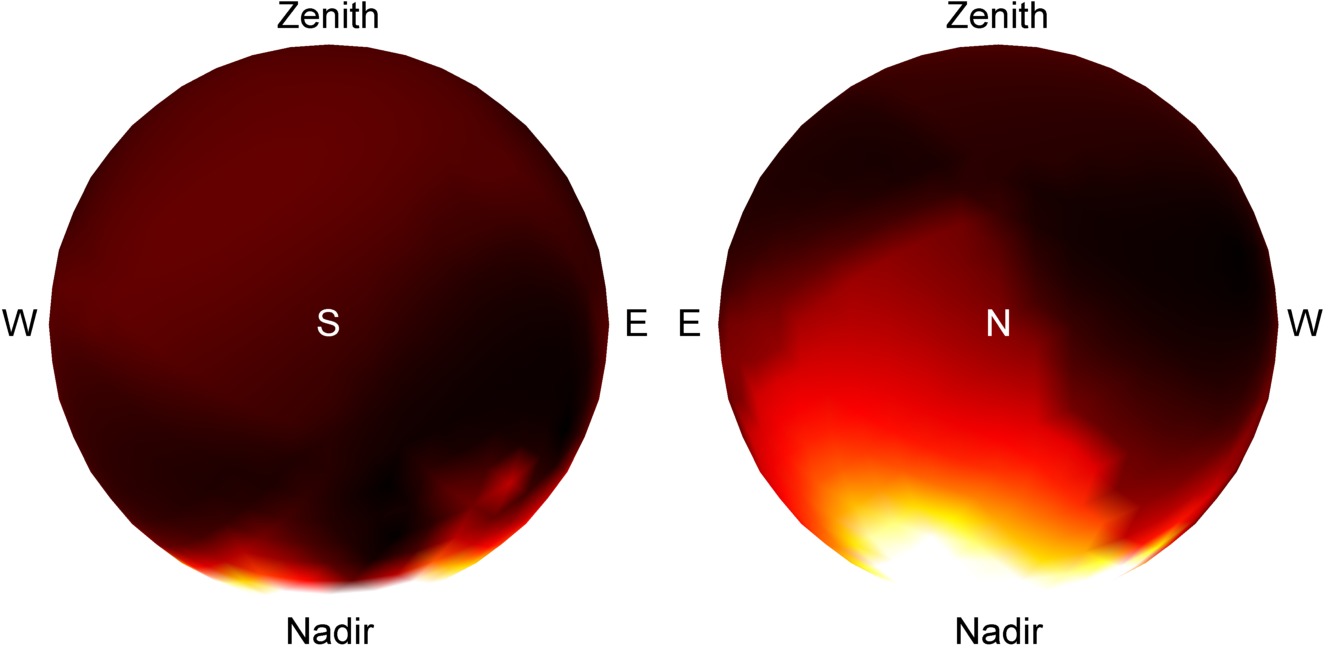
\includegraphics[width=.9\linewidth]{./figures/confidenceIntervals/20130824_10pm.png} \\
    \vspace{-.8em} \noindent\rule{\linewidth}{0.1pt}
    \begin{sideways}\begin{minipage}{.45\linewidth}\centering \scriptsize 11/06/2013 \\ 41\% sun visibility \vspace{5pt} \end{minipage}\end{sideways}
    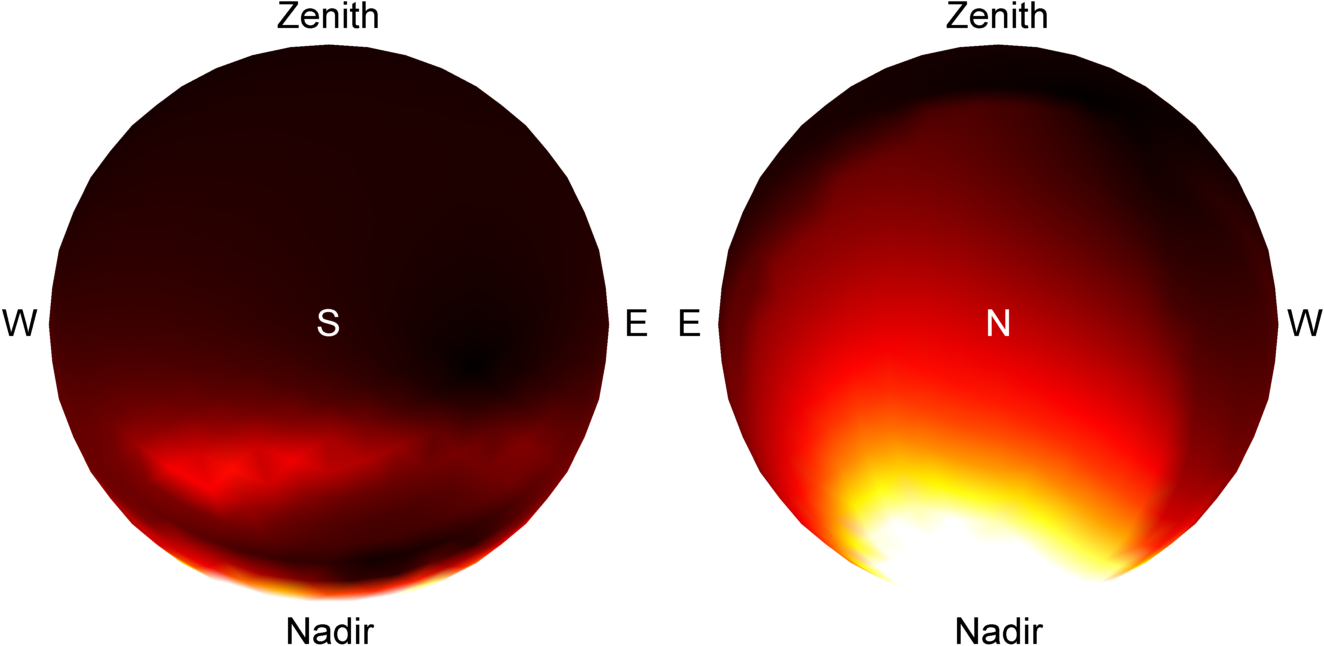
\includegraphics[width=.9\linewidth]{./figures/confidenceIntervals/20131106_10pm.png} \\
    \vspace{-.8em} \noindent\rule{\linewidth}{0.1pt}
    \begin{sideways}\begin{minipage}{.45\linewidth}\centering \scriptsize 11/08/2014 \\ 16\% sun visibility \vspace{5pt} \end{minipage}\end{sideways}
    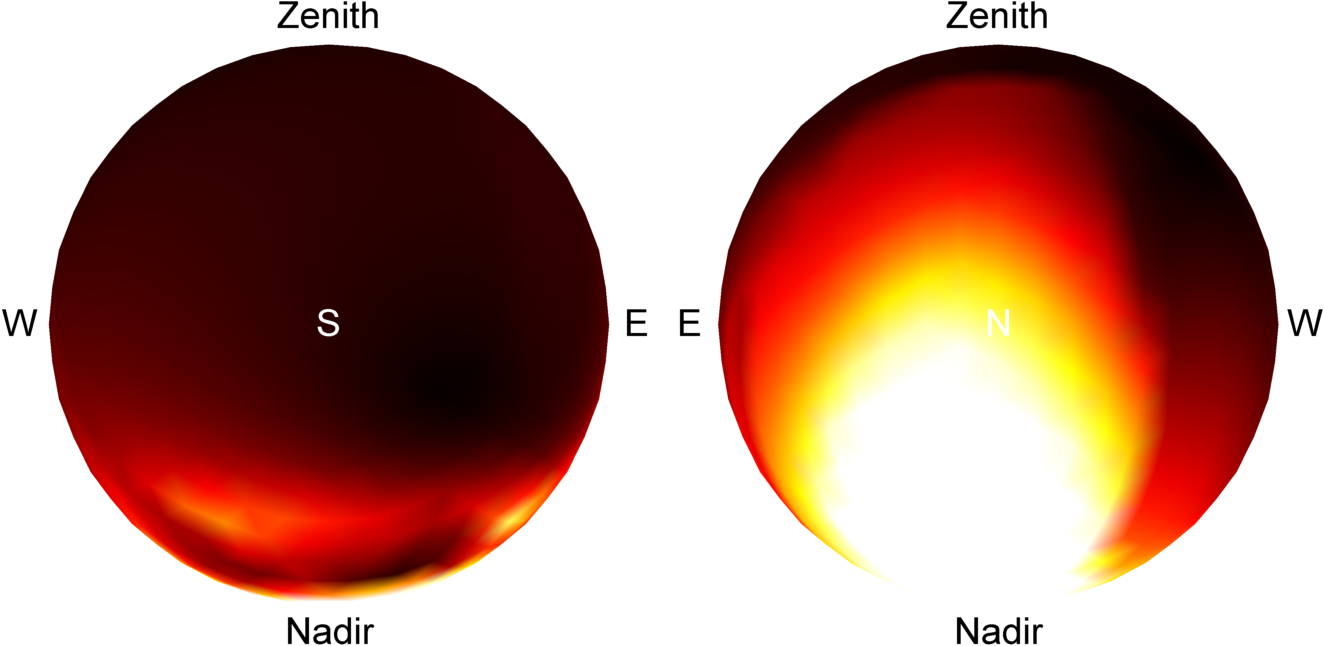
\includegraphics[width=.9\linewidth]{./figures/confidenceIntervals/20141108_10pm.png} \\
    \vspace{3mm}
    \includegraphics[width=1.01\linewidth]{./figures/confidenceIntervals/colorbar.png}
    \caption{Uncertainty in normal estimation with $\sigma=1\%$ is indicated by 95\% confidence intervals (in degrees), as a function of ground-truth surface normal. Results are shown for three different days in our dataset (same days as in fig.~\ref{fig:database}). The plots show the full sphere of normals from two different viewpoints: South (left), and North (right). Cardinal directions are shown for reference. The color-coding is indicated below the plots. See companion video for an animated version of these plots.}
    \label{fig:confidence-intervals}
\end{figure}

\begin{figure*}[t]
    \centering
    \includegraphics[width=.99\linewidth]{./figures/confidenceIntervals/sunVisibilityPlot-topHemisphere.pdf}
    \vspace{-2mm}
    \caption{Median confidence interval of normal estimates (red line) as a function of mean sun visibility over the course of the day for various values of $\sigma$. Our analysis predicts that normal reconstruction errors will likely be high if the sky is completely overcast (low sun visibility), or completely clear (high sun visibility). Good results can thus be expected in partially cloudy conditions, as shown in fig.~\ref{fig:cloud-cover}. The lower (upper) edge of each blue box indicates the 25th (75th) percentile. Statistics are computed only on normals pointing upwards to lessen ground effects.}
    \label{fig:cloud-cover-plot}
\end{figure*}


\subsubsection{Computing the stability of outdoor PS}

We aim to apply the stability analysis of sec.~\ref{sec:analysis} on all 23 days from our dataset, and on all possible normal directions. To do so, we consider each day independently, and first sample directions on the sphere by subdividing an icosahedron three times, yielding a set of 642 potential orientations $\mathcal{N} = \{\mathbf{n}_1, ..., \mathbf{n}_{642} \}$. Then, for each $\mathbf{n}_j \in \mathcal{N}$, we build the illumination matrix $\mathbf{L}$ in~\eqref{eqn:matrix-form}, given all 6 hours of data for that day. Finally, the 95\% confidence interval $\mathcal{C}_{\mathbf{n}_j}$ is computed using~\eqref{eqn:confidence-degrees}, indicating the uncertainty (possible reconstruction error) for that normal---the higher the interval, the less stable the solution.

To compute $\mathcal{C}_{\mathbf{n}_j}$, values for the noise level $\sigma$ and the surface albedo $\rho$ from \eqref{eqn:confidence-xyz} must be chosen. For the albedo, we will consider the best case with $\rho=1$. To set $\sigma$, we first render noise-less pixel values $\mathbf{b}_j$ using the (ground-truth) normal ${\bf n}_j$ and~\eqref{eqn:matrix-form}, with ${\bf L}$ including our entire collection of environment maps. All figures have been generated with $\sigma$ set at $1\%$ of the 95th percentile value of the resulting $\mathbf{b}_j$, unless otherwise stated. This particular value is chosen to yield a small, yet non-negligible, level of noise that is similar to that in previous work~\cite{klaudiny-prl-14}. The values of $\rho$ and $\sigma$ are kept constant in order to focus solely on the influence of lighting conditions, but could be set to match particular experimental conditions if needed.

Fig.~\ref{fig:confidence-intervals} shows the result of such an analysis on the three days of fig.~\ref{fig:database}. For each day, two sides of the sphere of normal directions are shown: seen from the South (left), and from the North (right). The spheres are color-coded according to the confidence interval $\mathcal{C}_\mathbf{n}$ for each normal direction. Note that vertex interpolation is used to display full spheres, but valid data is available only at vertices (thus the staircase effect in some plots).

At first glance, we notice that normals pointing down (towards Nadir) consistently have high confidence intervals, irrespective of the illumination conditions. The stability of outdoor PS on these normals is thus expected to be low. This behavior concords with expectation: normals pointing down define integration domains $\Omega_{\mathbf{n}}$ (see fig.~\ref{fig:normal-diagram}) which mostly include the ground, whose intensity does not vary spatially throughout the day. Another interesting observation from fig.~\ref{fig:confidence-intervals} is that the same normal exhibits different confidence intervals depending on the day. This raises the question: what is the relation between outdoor illumination conditions and uncertainty in the recovered surface normal?


\subsubsection{Influence of cloud cover}
\label{sec:cloud-cover-results}

It is already apparent from fig.~\ref{fig:confidence-intervals} that cloud coverage has an effect on the uncertainty of normal reconstruction, since an overcast day (last row) clearly does not behave the same way as a day with light clouds (top row). Here, we present a more systematic analysis of the influence of cloud coverage. To control for the effect of the sun elevation (which will be explored in sec.~\ref{sec:sun-elevation-results}), the analysis is performed on days with similar sun elevations by keeping only the skies captured in October and November.

We approximate cloud coverage by computing the fraction of time that the sun is visible, \ie, that it fully shines on the scene, for a given day. To do so, we simply find the brightest spot in a sky image, and determine that the sun shines on the scene if the intensity of the brightest pixel is greater than $20\%$ of the maximum sun intensity---we determined empirically that this is the point at which the sun is bright enough to start creating cast shadows. Cloud coverage is represented by computing the mean sun visibility for a given day. A value of less than 10--15\% would indicate a mostly overcast sky, while skies are mostly clear with values above 85--90\%.

\begin{figure}[t]
    \centering
    \begin{sideways}\begin{minipage}{.45\linewidth}\centering \scriptsize Clear (85-100\%)\vspace{5pt} \end{minipage}\end{sideways}
    \includegraphics[width=.9\linewidth]{./figures/confidenceIntervals/clear-mean_10pm.png} \\
    \vspace{-.8em} \noindent\rule{\linewidth}{0.1pt}
    \begin{sideways}\begin{minipage}{.45\linewidth}\centering \scriptsize Mixed Clear (50-85\%)\vspace{5pt} \end{minipage}\end{sideways}
    \includegraphics[width=.9\linewidth]{./figures/confidenceIntervals/mixed-clear-mean_10pm.png} \\
    \vspace{-.8em} \noindent\rule{\linewidth}{0.1pt}
    \begin{sideways}\begin{minipage}{.45\linewidth}\centering \scriptsize Mixed Overcast (15-50\%)\vspace{5pt} \end{minipage}\end{sideways}
    \includegraphics[width=.9\linewidth]{./figures/confidenceIntervals/mixed-overcast-mean_10pm.png} \\
    \vspace{-.8em} \noindent\rule{\linewidth}{0.1pt}
    \begin{sideways}\begin{minipage}{.45\linewidth}\centering \scriptsize Overcast (0-15\%)\vspace{5pt} \end{minipage}\end{sideways}
    \includegraphics[width=.9\linewidth]{./figures/confidenceIntervals/overcast-mean_10pm.png} \\
    \vspace{3mm}
    \includegraphics[width=1.01\linewidth]{./figures/confidenceIntervals/colorbar.png}
    \caption{Influence of cloud cover on the 95\% confidence intervals with $\sigma=1\%$. Each row shows a different type of sky, based on sun visibility. For example, the top row shows confidence intervals averaged over all days with direct sun visibility in the range 85\%-100\%. The averaged days presented similar sun elevations. As with fig.~\ref{fig:confidence-intervals}, the plots show the full sphere of normals from two different viewpoints: South (left), and North (right).}
    \label{fig:cloud-cover}
\end{figure}

The relation between sun visibility and the confidence interval $\mathcal{C}_\mathbf{n}$ is shown in fig.~\ref{fig:cloud-cover-plot}. Normal reconstruction errors will likely be quite high in two situations: when the sky is completely overcast (low sun visibility), or completely clear (high sun visibility). Interestingly, good reconstruction results are expected for a wide range of cloud coverage conditions, ranging from 10--90\% mean sun visibility.

These results are corroborated by fig.~\ref{fig:cloud-cover}, which shows the confidence intervals themselves on a plot similar to fig.~\ref{fig:confidence-intervals}. Results there are presented by averaging the intervals of skies belonging to four groups: overcast (0--15\%), mixed overcast (15--50\%), mixed clear (50--85\%), and clear (85--100\%) days. Again, high uncertainty results are visible for the two extreme cases of fully overcast and fully clear days, while the remainder indicate more stable solutions.

% TODO: add figure to illustrate this (maybe)?
The improved conditioning in mixed skies is explained by the following key observation: cloud cover shifts the mean light vectors ${\bf \bar l}_t$ towards zenith and away from sun trajectory in the sky. Therefore, even when the sun moves along a trajectory that nearly lies on a 3D plane, as shown in fig.~\ref{fig:mlv}, cloud cover effectively causes an {\em out-of-plane} shift of the mean light vectors, making reconstruction possible.

\begin{figure}
    \centering
    \includegraphics[width=\linewidth]{./figures/mlvFig/mlvFig.pdf}
    \caption{Cloud effect on the mean light direction over one day: while the sun path (orange) yields nearly co-planar directions of illumination, the mean light directions (red dots) provide a much more varied set (data from 11/06/2013, 2nd row of fig.~\ref{fig:database}).}
    \label{fig:mlv}
\end{figure}

This key observation also demonstrates the advantages of adopting more elaborate illumination models (\eg, \cite{yu-iccp-13}). For instance, the simpler point light model was used in \cite{shen-pg-14} to study the conditioning of outdoor PS. Because the atmospheric component is not modeled, the conclusion was that single-day reconstruction breaks down in two cases of nearly coplanar sun directions: closer to the poles near the winter solstice, and worldwide near an equinox. Our results suggest that more attention should be placed on the illumination model, without focusing exclusively on the sun.

\subsubsection{Influence of sun elevation}
\label{sec:sun-elevation-results}

We also hypothesized the position of the sun to have an important effect on the ability to recover surface normals outdoors. Since our dataset is already aligned in terms of sun azimuths (see sec.~\ref{sec:dataset}), we now analyze the influence of sun elevation. For this purpose, we retain only the days for which the sun visibility was between 15--85\% of the time. We then compute the relation between sun elevation and expected reconstruction confidence, as illustrated in fig.~\ref{fig:sun-elevation-plot}.

Sun elevation does appear to have an influence, with higher sun elevations resulting in slightly increased uncertainty than when the sun is lower in the sky. However, the impact is less drastic than that of cloud cover from sec.~\ref{sec:cloud-cover-results}. These results can be explained, at least in part, by the smaller sun-zenith shift introduced by cloud cover when the sun is already high in the sky; therefore, smaller improvements in conditioning are obtained.

Our data-driven analysis shows that higher sun elevations---predicted as preferable by the analysis in~\cite{shen-pg-14}---are in fact not necessarily optimal when taking more elaborate illumination models into account.


% Section 3 has a note about non-coplanar sun directions  vs  non-coplanar mean light vectors (zenith, sun elevation),


\subsubsection{Analyzing full objects}

So far, our analysis has focused solely on one patch (one normal direction) at a time. But can we also say something about an entire object? Clearly, a full answer to this question would require analyzing non-local effects such as occlusions, inter-reflections, cast shadows, etc. However, we hypothesize that a simpler analysis ignoring these effects can still provide useful results. We therefore predict the performance of an outdoor PS algorithm by computing the expected value of the confidence interval, $\mathbb{E}_{\bf n}[\mathcal{C}_{\bf n}]$, over an entire object; expectation over the normal vector is computed using a prior distribution taken from a simpler convex shape (\eg, a sphere). Fig.~\ref{fig:objects} shows the expected reconstruction performance for two objects: a bottle, and the bunny. Overall, surface reconstruction performance is expected to be best when objects face south (\ie, the sun).

\begin{figure}[t]
    \centering
    \includegraphics[width=\linewidth]{./figures/confidenceIntervals/sunElevationPlot-topHemisphere.pdf}
    \caption{Median confidence interval of normal estimates (red line) as a function of maximum sun elevation over the course of the day for various values of $\sigma$. Although the effect is not as significant as with cloud cover, we anticipate a small decrease in performance at higher sun elevations. The lower (upper) edge of each blue box indicates the 25th (75th) percentile. Statistics are computed only on normals pointing upwards to lessen ground effects.}
    \label{fig:sun-elevation-plot}
\end{figure}

% \begin{figure}[t]
%     \centering
%     \begin{sideways}\begin{minipage}{.45\linewidth}\centering \scriptsize Low elevation \vspace{5pt} \end{minipage}\end{sideways}
%     \includegraphics[width=.9\linewidth]{./figures/confidenceIntervals/elevation-low-mean_10pm.png} \\[2mm]
%     \begin{sideways}\begin{minipage}{.45\linewidth}\centering \scriptsize High elevation \vspace{5pt} \end{minipage}\end{sideways}
%     \includegraphics[width=.9\linewidth]{./figures/confidenceIntervals/elevation-high-mean_10pm.png} \\[3mm]
%     \includegraphics[width=\linewidth]{./figures/confidenceIntervals/colorbar.png}
%   \caption{Influence of sun elevation on the 95\% confidence intervals with $\sigma=1\%$. The top plot shows the mean, per-normal, confidence intervals obtained for mixed skies with low sun elevation. The bottom plot shows the same data, but for mixed skies with high sun elevation. As in fig.~\ref{fig:confidence-intervals}, the plots show the full sphere of normals from two different viewpoints: South (left), and North (right). Cardinal directions are shown for reference. The color-coding is indicated below the plots.}
%   \label{fig:sun-elevation}
% \end{figure}

\begin{figure}[t]
    \centering
    \includegraphics[width=\linewidth]{./figures/objectFig/objectFigNoise.pdf}
    \caption{Predicting object reconstruction performance for the 08/24/2013 dataset. These curves show the mean surface reconstruction variance for two objects: a bottle (blue) and the bunny (red). Irrespective of the noise level, surface reconstruction performance is expected to be best when the objects face south.}
    \label{fig:objects}
\end{figure}

\subsection{Validation on real object images}
\label{sec:validation}

The analysis performed on our dataset indicates that surface patches may be better reconstructed in certain conditions, dependent upon cloud coverage, sun elevation, and the orientation of the patch itself. At the time of this writing, a thorough validation on real outdoor images of different objects is currently under development. This section reports preliminary results on real outdoor images of an owl statuette (fig.~\ref{fig:reconstruction:example_envmaps}), which was scanned with a Creaform MetraSCAN at a resolution of 0.05mm to provide a reference of true surface orientation.

\begin{figure*}[!ht]
    \centering
    \setlength{\tabcolsep}{0pt}
    \newcommand{\customwidth}{.08\linewidth}
    \begin{tabular}{@{}rcccccccccccc@{}}
    &
    \begin{minipage}{\customwidth}\centering\scriptsize 10:30 \end{minipage} &
    \begin{minipage}{\customwidth}\centering\scriptsize 11:00 \end{minipage} &
    \begin{minipage}{\customwidth}\centering\scriptsize 11:30 \end{minipage} &
    \begin{minipage}{\customwidth}\centering\scriptsize 12:00 \end{minipage} &
    \begin{minipage}{\customwidth}\centering\scriptsize 12:30 \end{minipage} &
    \begin{minipage}{\customwidth}\centering\scriptsize 13:00 \end{minipage} &
    \begin{minipage}{\customwidth}\centering\scriptsize 13:30 \end{minipage} &
    \begin{minipage}{\customwidth}\centering\scriptsize 14:00 \end{minipage} &
    \begin{minipage}{\customwidth}\centering\scriptsize 14:30 \end{minipage} &
    \begin{minipage}{\customwidth}\centering\scriptsize 15:00 \end{minipage} &
    \begin{minipage}{\customwidth}\centering\scriptsize 15:30 \end{minipage} &
    \begin{minipage}{\customwidth}\centering\scriptsize 16:00 \end{minipage}
    \\
    \begin{sideways}\begin{minipage}{\customwidth}\centering \scriptsize illumination \\ 43\% sun vis. \\ \vspace{5pt} \end{minipage}\end{sideways} &
    \includegraphics[width=\customwidth]{./figures/reconstruction/envmaps/20141011_102928.jpg} &
    \includegraphics[width=\customwidth]{./figures/reconstruction/envmaps/20141011_110128.jpg} &
    \includegraphics[width=\customwidth]{./figures/reconstruction/envmaps/20141011_112928.jpg} &
    \includegraphics[width=\customwidth]{./figures/reconstruction/envmaps/20141011_120128.jpg} &
    \includegraphics[width=\customwidth]{./figures/reconstruction/envmaps/20141011_122929.jpg} &
    \includegraphics[width=\customwidth]{./figures/reconstruction/envmaps/20141011_130128.jpg} &
    \includegraphics[width=\customwidth]{./figures/reconstruction/envmaps/20141011_132928.jpg} &
    \includegraphics[width=\customwidth]{./figures/reconstruction/envmaps/20141011_135928.jpg} &
    \includegraphics[width=\customwidth]{./figures/reconstruction/envmaps/20141011_142928.jpg} &
    \includegraphics[width=\customwidth]{./figures/reconstruction/envmaps/20141011_145928.jpg} &
    \includegraphics[width=\customwidth]{./figures/reconstruction/envmaps/20141011_152928.jpg} &
    \includegraphics[width=\customwidth]{./figures/reconstruction/envmaps/20141011_155928.jpg}
    \\
    \begin{sideways}\begin{minipage}{.106\linewidth}\centering \scriptsize object capture \\ \vspace{1em} \vspace{5pt} \end{minipage}\end{sideways} &
    \includegraphics[width=\customwidth]{./figures/reconstruction/object/103307.jpg} &
    \includegraphics[width=\customwidth]{./figures/reconstruction/object/110346.jpg} &
    \includegraphics[width=\customwidth]{./figures/reconstruction/object/113346.jpg} &
    \includegraphics[width=\customwidth]{./figures/reconstruction/object/120346.jpg} &
    \includegraphics[width=\customwidth]{./figures/reconstruction/object/123346.jpg} &
    \includegraphics[width=\customwidth]{./figures/reconstruction/object/130215.jpg} &
    \includegraphics[width=\customwidth]{./figures/reconstruction/object/133215.jpg} &
    \includegraphics[width=\customwidth]{./figures/reconstruction/object/135615.jpg} &
    \includegraphics[width=\customwidth]{./figures/reconstruction/object/143215.jpg} &
    \includegraphics[width=\customwidth]{./figures/reconstruction/object/150215.jpg} &
    \includegraphics[width=\customwidth]{./figures/reconstruction/object/153215.jpg} &
    \includegraphics[width=\customwidth]{./figures/reconstruction/object/160215.jpg}

    \end{tabular}
    \caption{Real outdoor HDR images of owl statuette and corresponding HDR environment maps (top row) providing synchronized, high-fidelity estimates of illumination conditions. All images were acquired on 10/11/2014 and tone-mapped for display only (with $\gamma = 1.6$). The sun visibility was 43\% on this day. }
    \label{fig:reconstruction:example_envmaps}
    \vspace{-1em}
\end{figure*}

We oriented this owl statuette towards south and took 66 HDR captures using a Canon EOS Rebel SL1 between 10h30 and 16h30, local time, in Quebec City. These captures were synchronized with the HDR environment maps described in sec.~\ref{sec:introduction}, providing high fidelity estimates of the illumination conditions for each image, as shown in fig.~\ref{fig:reconstruction:example_envmaps}. The laser scan was then manually aligned to these images.

A simple outdoor PS algorithm was run on evenly distributed patches on the owl images. For each patch, the surface normal is obtained as to minimize the rendering error given by the model in~\eqref{eqn:matrix-form}, in a least-squares sense. Since this estimation problem is nonlinear on the normal ${\bf n}$, a solution is computed via exhaustive search on a set of 271 candidate orientations for the light hemisphere $\Omega_{\bf n}$. Given $\Omega_{\bf n}$, a candidate solution ${\bf x}$ is obtained via linear least squares. For the best solution, an estimation error, in degrees, is computed using the reference normal from the laser scan. The uncertainty measure (confidence interval $\mathcal{C}_{\bf n}$) derived in sec.~\ref{subsec:measure_uncertainty} is also computed for each patch.

Results from this quantitative evaluation are given in fig.~\ref{fig:reconstruction:results}. As shown on the left, normals pointing upwards are generally recovered more accurately than normals pointing downwards. This is in concordance with the predicted confidence intervals shown on the right in fig.~\ref{fig:reconstruction:results}. The behavior of the reconstruction error is, in general, well predicted by the confidence intervals.
% Note however that the ground truth normals were aligned with the images manually, therefore slight misalignments could explain discrepancies.


\begin{figure}[t]
    \centering
    \newcommand{\customwidthres}{0.45\linewidth}
    \begin{tabular}{cc}
        \scriptsize Angular differences to ground truth & \scriptsize Predicted 95\% confidence intervals \\
        \includegraphics[width=\customwidthres]{./figures/reconstruction/owl_delta_gt.png} &
        \includegraphics[width=\customwidthres]{./figures/reconstruction/owl_confint.png}
        \begin{picture}(0,0)
            \put(-155,-2){\includegraphics[height=1.5cm]{./figures/reconstruction/owl_sphere_dgt.png}}
            \put(-35,-2){\includegraphics[height=1.5cm]{./figures/reconstruction/owl_sphere_ci.png}}
        \end{picture}
    \end{tabular}
    \includegraphics[width=1.01\linewidth]{./figures/reconstruction/colorbar.png}
    \caption{Quantitative validation on images of a real object. Evenly distributed patches of the owl images were used to perform a simple calibrated outdoor PS algorithm. Error estimates of the surface normals are reported on the left using the reference surface orientation in the laser scan. The predicted 95\% confidence intervals $\mathcal{C}_\mathbf{n}$ from \eqref{eqn:confidence-degrees} are shown on the right. A few large estimation errors on the left image may be caused by imperfect alignment between the scanned model and the images. Insets in the lower right corner show the recovered normals mapped to the south hemisphere. Normals in dark blue means no data available.}
    \label{fig:reconstruction:results}
\end{figure}


\subsubsection{Discussion and future work}
\label{sec:iccp-discussion}

This paper has presented the first data-driven analysis of the expected behavior of PS under outdoor illumination. In this scenario, we have no control over the illumination conditions themselves, so existing methods to determine an optimal illumination setup~\cite{drbohlav-iccv-05,klaudiny-prl-14} cannot be applied. Our goal is, therefore, to reveal natural factors that distinguish good and unfavorable daylight conditions for outdoor PS.

The recent work of Shen et al.~\cite{shen-pg-14} presents an insightful, theoretical analysis of the conditioning of outdoor PS using the standard illumination model with a point light source. Their work suggests that PS reconstruction becomes unstable in two cases of nearly planar sun motion: near the poles during the winter solstices, and worldwide near the equinoxes. However, these conclusions are drawn based on a simple illumination model that focuses exclusively on direct sun light, without considering other atmospheric components. Our approach is fundamentally different in that we adopt a more realistic illumination model and then follow a data-driven approach to investigate the conditioning of outdoor PS. We identify not only solar, but also atmospheric and object-intrinsic factors that contribute to stability, or uncertainty, in the photometric reconstruction.

% mention PS in one vs multiple days above?

To achieve our goal, we exploit a large database of outdoor HDR environment maps that provide a rich sampling of the natural variability in outdoor illumination. To make comprehensive use of this dataset, our photometric model considers not only direct sun illumination, but also the full atmospheric (sky) component and an additional ground effect. We then derive a theoretical analysis to investigate the stability of surface normal reconstruction, as measured by an intuitive angular confidence interval. Our empirical analysis reveals how reconstruction is affected by surface orientation, cloud coverage, and sun elevation. Our preliminary quantitative experiments corroborate the predictions with actual reconstruction results.

%There is an interesting relationship between our work and the recent work of Shen et al.~\cite{shen-pg-14}. Their work uses a geometrical analysis to show that, as a function of time of year and latitude, the sun path is sometimes \emph{not} planar and it alone can be used to estimate surface normals reliably. In our case, we employ a data-driven approach which considers the impact of the entire sky hemisphere (including the sun position), the normal direction, camera parameters, and surface reflectance. \todo{Write this when we have more details about the influence of the sun elevation}.

In short, our analysis revealed the following important observations of direct practical value. We show that better stability can be achieved when:
\begin{enumerate}[nosep]
    \item surface patches are oriented South and above the horizon: since our data was captured in the Northern Hemisphere, these are the patches (normals) that ``see'' the sun while it moves during the day;
    \item the sky is partially cloudy throughout the day: this resulted in improved stability than either completely sunny, or completely overcast days;
    \item the sun is lower in the sky: this resulted, on average, in slightly better performance than with days where the sun is higher in the sky.
\end{enumerate}
% In short, our analysis revealed important observations of direct practical value. First, better stability is typically observed for surface patches oriented south and above the horizon. Since our data was captured in the Northern Hemisphere, these are the patches (normals) that ``see'' the sun while it moves during the day. Second, partially cloudy conditions resulted in better stability than either completely sunny, or completely overcast days. Third, days with lower sun elevations yielded, on average, slightly better performance than days with higher sun elevations.
While these observations might seem intuitive to an experienced practitioner, as far as we know, our work is the first attempt to confirm or contradict such intuition in outdoor PS. For instance, a common belief has been that clear days were preferable~\cite{yu-iccp-13,inose-tcva-13,ackermann-cvpr-12,abrams-eccv-12}, instead of mixed weather.

Another goal of this paper has been to inform future research in outdoor PS. Clearly, a better understanding of the sources of uncertainty is useful in developing better reconstruction algorithms (\eg, better informed regularization). Despite the interesting observations above, this work still has some limitations that also open the way to interesting future work. First, it would be interesting to explore the correlation between the predicted reconstruction performance (\eg, fig.~\ref{fig:objects}) and the performance of an actual outdoor photometric stereo algorithm such as~\cite{yu-iccp-13}. Second, our analysis assumes white Gaussian noise, for practical purposes; more realistic noise models for HDR photography should be investigated. Third, our current analysis does not model random perturbations in the light probes themselves (\ie,~${\bf L}$). These are interesting extensions that increase the complexity of our derivations above and, thus, are left as future work. Finally, some seasons are not well represented in our dataset yet. We plan on continuing data capture to further enrich this database of outdoor environment maps.


\section{$x$-hour Outdoor Photometric Stereo}
\label{3dv15}

Best theoretical reconstruction performance.
%%!TEX root = main.tex


\section{Outdoor PS conditioning}
\label{sec:sensitivity-analysis}

In the following, we consider a small planar surface patch with normal vector ${\bf n}$ and Lambertian reflectance with albedo~$\rho$. As discussed in~\cite{holdgeoffroy-iccp-15,hung-wacv-15}, the lighting contribution of an environment map to a Lambertian surface patch can be formulated as in an equivalent problem with a single point light source $\bar{\mathbf{l}} \in \mathbb{R}^3$. This vector is the mean of the light vectors computed over the hemisphere of incoming light directions defined by ${\bf n}$. This virtual point light source $\bar{\mathbf{l}}$ is henceforth referred to as the {\em mean light vector} (MLV). It is important to note that, as opposed to the traditional PS scenario where point light sources are fixed and thus independent of ${\bf n}$, here the {\em per-pixel} MLV is a function of $\mathbf{n}$. Thus, patches with different orientations define different sets of MLVs (as discussed later and shown in fig.~\ref{fig:realShiftNormal}).

Given multiple images of the same patch, taken at different times, we collect all photometric constraints for that patch and obtain the PS equation in matrix form:
%
\begin{equation}
\mathbf{b} =
\begin{bmatrix}
 b_1 \\ b_2 \\ \vdots \\ b_T
\end{bmatrix}
= 
\begin{bmatrix}
 {\bf \bar l}_1^T \\ {\bf \bar l}_2^T \\ \vdots \\ {\bf \bar l}_T^T
\end{bmatrix}
{\bf x} = \mathbf{L} \mathbf{x} \,,
\label{eqn:matrix-form}
\end{equation}
%
where $b_i \in \mathbb{R}$ are the observed pixel intensities, and ${\bf x} \in \mathbb{R}^3$ is the surface normal ${\bf n}$ scaled by $\rho$.

Let $\hat{{\bf x}}=({\bf L}^T{\bf L})^{-1}{\bf L}^T{\bf b}$ denote the least-squares solution of~\eqref{eqn:matrix-form}. A 95\% confidence interval for normal ${\bf x}$ is given by 
%
\begin{equation}
\hat{\mathbf{x}} \pm \bolddelta \,, \quad \text{with } \delta_k = 1.96 \frac{\sigma}{\rho}\lambda_k \,,
\label{eqn:confidence-xyz}
\end{equation}
%
where $\sigma$ is the camera noise level and $\lambda_k$ is the square root of the $k$-th element on the diagonal of $({\bf L}^T{\bf L})^{-1}$~\cite{hastie-book-09}. 

% A more intuitive measure of uncertainty in the estimate $\hat{{\bf n}}$ is obtained by considering angular distances $\theta$ in degrees, 
% % 
% \begin{equation}
% \theta^\pm = \cos^{-1}({\bf \hat n}^T{\bf \hat n}^\pm)\,, 
% \quad \text{where }
% {\bf \hat n}^\pm = \frac{{\bf \hat n} \pm \bolddelta}{\lVert{\bf \hat n} \pm \bolddelta \rVert}.
% \label{eqn:angular-dist}
% \end{equation}
% %
% Our measure of uncertainty, or stability, in the estimation of ${\bf \hat n}$ is then defined as the confidence interval \mbox{$\mathcal{C}_{\bf n} = [ 0, \max(\theta^\pm) ]$} in degrees.

% In the analysis below, we often take the estimate ${\bf \hat n}$ to be the ground truth normal ${\bf n}$ of a simulated (synthetic) surface patch; this corresponds to the result of an ideal algorithm. We then evaluate the confidence interval for this normal using a set of real, outdoor environment maps with associated stability parameters $\lambda_k$ as in~\eqref{eqn:confidence-xyz}. The result is a measure of the uncertainty in the reconstruction that an actual outdoor PS algorithm would provide on that particular set of illumination conditions, and surface orientation. As in~\cite{holdgeoffroy-iccp-15}, our simulations below consider synthetic surface patches with albedo $\rho = 1$ and a small, non-negligible noise level $\sigma$ at $1\%$ of the maximum pixel value.

From \eqref{eqn:confidence-xyz}, note that the only light-dependent stability factor in the confidence interval $\bolddelta$ is $\lambda_k$; the other two factors are related to the camera ($\sigma$), and surface reflectance~($\rho$). In this paper, we analyze the maximum uncertainty \mbox{$\lambda_\text{max} = \max_k(\lambda_k)$}, as a conservative performance measure that is independent of albedo and sensor noise; $\lambda_\text{max}$ is a {\em maximum noise gain} factor, \ie, the intensity of noise amplification in the solution. Here, we are interested in (\emph{i}) investigating how the noise gain $\lambda_\text{max}$ is influenced by the duration of outdoor data capture, and in (\emph{ii}) identifying specific changes, or {\em events}, in outdoor lighting that are associated with more stable PS solutions (smaller $\lambda_\text{max}$).

To make our analysis tractable, we do not model cast shadows and inter-reflections. In addition, we assume that the sky hemisphere (around zenith) provides the dominant part of incoming light. Unless stated otherwise, our simulations consider a day near an equinox, which corresponds to the worst case scenario with coplanar sun directions~\cite{shen-pg-14}.


\section{$x$-hour outdoor PS}
%\section{Time interval analysis}
\label{sec:analysis}

This section provides the first answers to the questions raised above by looking at collections of mean light vectors (MLVs) from both simulated and real sky data. The main goal is to analyze the behavior of the illumination factors $\lambda_k$ (and associated confidence interval) of normal estimation. More specifically, we investigate numerical stability (MLV coplanarity) as a function of the apparent sun motion and cloud coverage within capture intervals of different durations, containing different atmospheric events. We also compare the resulting performance measures of $x$-hour outdoor PS to those of full-day outdoor PS.

% Here our goal is to answer the questions: \emph{what} are the important changes, or {\em events}, in outdoor lighting that affect $\lambda_k$? What is the minimum duration of data capture, containing one or more of such events, that can lead to performance similar to that of full-day PS?

% -----------------------------------------------------------------------------
\begin{figure}[t]
\centering
\includegraphics[width=.8\columnwidth]{diagram_MLVshift3}
\caption{Impact of cloud coverage on the numerical conditioning of outdoor PS: clear (a) and overcast (b) days present MLVs with stronger coplanarity; in partly cloudy days (c) the sun is often obscured by clouds, which may lead to out-of-plane shifts of MLVs.}
\label{fig:MLVshift}
\end{figure}
% -----------------------------------------------------------------------------
% -----------------------------------------------------------------------------
\begin{figure*}[t]
\centering
\includegraphics[width=.32\textwidth]{v123gainSurf} \ \ \ %\\[3mm]
\includegraphics[width=.32\textwidth]{v123gain1Arc} \ \ \ %\\[3mm]
\includegraphics[width=.32\textwidth]{v123gain2Shift}
\caption{Simulated noise gain $\lambda_{\max}(\theta_a,\theta_e)$ as a function of solar arc $\theta_a$ and MLV shift (elevation) angle $\theta_e$. See discussion in the text.}
\label{fig:v123gain}
\end{figure*}
% -----------------------------------------------------------------------------

\subsection{Cloud coverage and MLV shifting}
\label{subsec:mlv-clouds}

As shown in~\cite{holdgeoffroy-iccp-15}, with data captured under clear skies, the MLVs of the model above will point nearly towards the sun, from which arrives most of the incoming light. Thus, near an equinox (worldwide), the resulting set of MLVs are nearly coplanar~\cite{shen-pg-14}, resulting in poor performance, fig.~\ref{fig:MLVshift}(a). For a day with an overcast sky, performance is also poor because the set of MLVs are nearly colinear and shifted towards the patch normal ${\bf n}$, fig.~\ref{fig:MLVshift}(b). Finally, in partly cloudy days (mixed skies), the sun is often obscured by clouds and such occlusion shifts some MLVs away from the solar plane, improving numerical stability, fig.~\ref{fig:MLVshift}(c). 

% NOT SURE ABOUT THIS ANYMORE:
% This improvement in conditioning is more significant with lower sun elevations, as the MLVs are shifted towards zenith.


\subsection{Solar arcs and MLV elevation}
\label{subsec:solararcs-mlvelevation}

%If we assume equinox, then the sun actually moves on a plane worldwide (i.e. independent of latitude) and is also visible 12 hours worldwide (although terrain and atmosphere play a small role and change that). Thus, this simulation requires the equinox assumption. What does vary with latitude (at equinox) is: (1) the inclination of the solar plane, and (2) the frequency of cloud coverage (if the sun is lower in the sky most of the day). Anything else?

Here, we seek to provide a sense of the minimal length of solar arc and amount of out-of-plane MLV shift required in single-day outdoor PS.

Assuming a day near an equinox, the apparent sun trajectory worldwide describes an arc $\theta_a$ within the solar plane of about $15^\circ$ per hour. We now use this observation to evaluate the numerical stability of outdoor PS for data capture intervals (solar arcs) of different lengths. Considering a partly cloudy sky, we also investigate the interaction of solar arc and cloud coverage; we quantify performance as a function of both acquisition time (solar arc $\theta_a$) and amount of out-of-plane MLV shift (elevation angle $\theta_e$) introduced by clouds.

A simple and effective way to investigate conditioning with different capture scenarios is to consider a simulation with the minimum number of three MLVs, as required for outdoor PS using~\eqref{eqn:matrix-form}. We simulate solar arcs $\theta_a$ of different lengths by defining two MLVs on a reference solar plane, with the third MLV presenting varying elevation $\theta_e$ away from this plane, as illustrated in fig.~\ref{fig:MLVshift}(c). The actual orientation of the solar plane varies with the latitude of the observer; thus, we represent MLV shift relative to this plane.

The numerical conditioning of outdoor PS, as observed with different configurations for these three MLVs, is then scored using the noise gain~$\lambda_{\max}$ (sec.~\ref{sec:sensitivity-analysis}). This measure is independent of albedo and sensor noise; it is also related to the condition number of the illumination matrix ${\bf L}$ in~\eqref{eqn:matrix-form}.

% Lower bound as MLV intensity is reduced by cloud coverage; thus MLV elevation need to be higher, actually.

% define full day as 6-hour outdoor PS (shadowing concerns)?

We compute~$\lambda_{\max}(\theta_a,\theta_e)$ for solar arcs $\theta_a$ of up to 6 hours ($90^\circ$) and MLV elevations $\theta_e$ up to $90^\circ$. For simplicity, we consider triplets of unit-length MLVs---thus, conditioning depends on the magnitude $\sin(\theta_e)$ of the out-of-plane component of the third MLV. Clearly, the optimal noise gain~$\lambda_{\max} = 1$ is obtained when the MLVs are mutually orthogonal ($\theta_a = \theta_e = 90^\circ$).

Fig.~\ref{fig:v123gain}(a) shows that the noise gain $\lambda_{\max}$ drops quickly to under 6 for capture intervals at just above 1 hour and for MLV shifts $\theta_e > 15^0$. This result suggests that even the performance of 1-hour PS can be acceptable with small levels of sensor noise $\sigma$ and high surface reflectance $\rho$. To ease visualization, figs.~\ref{fig:v123gain}(b,c) show cross sections of the $\lambda_{\max}(\theta_a,\theta_e)$ gain surface for a constant shift or solar arc.

A second important prediction from fig.~\ref{fig:v123gain}, considering (more realistic) small to moderate amounts of MLV shifts $\theta_e \leq 40^\circ$, is that conditioning will improve very little for data capture intervals above 3 hours ($45^\circ$ solar arcs). Reducing data capture from 3 to 2 hours would lead to an additional increase in uncertainty ($\lambda_{\max}$) of less than $30\%$ (from about 2.8 to nearly 3.6). Still, 2-hour outdoor PS with noise gains under $4\times$ may be possible if an MLV shift of $\theta_e > 20^\circ$ is introduced by atmospheric events during capture. Uncertainty in the results of 1-hour outdoor PS would be about 5 to 7 times that of full-day (6-hour) outdoor PS.


\subsection{MLV shifts in real sky probes}

% how much MLV shift is expected?
% but how much uncertainty can we expect? look into real sky probes...
% Here we evaluate the actual noise gain from real data... 
% pick days near equinox to isolate shifting due to clouds only (really needed?)
% TODO: What happens with natural sun elevation in summer (non-equinox), high-latitude? sun declination angle of $23.5^\circ$. The other two vectors are always on plane!

% what we do: look at gain to infer elevation, we fit solar arc for clear sky, look at orthogonal component of MLVs
% for each normal visible to the camera, we plot the best gain computed from the solar plane and a third MLV
% does enough shift really happen? how much shift and for which normals?
% average/pattern over multiple days?

While the analysis above suggests that outdoor PS may be possible with a capture interval of only about 1 to 3 hours, it does not answer whether it is possible to observe an adequate amount of MLV shift (elevation away from solar plane) within a single partly cloudy day. In the following, we analyze the shifting (coplanarity) of real MLVs obtained from a database of real environment maps (sky probes)~\cite{holdgeoffroy-iccp-15}.

% MLV shifting depends on which portion of the sky the normal (patch) sees.
% shifting varies with normal (examples, more in suppl video)
% dimming in overcast (early morning/afternoon) affects conditioning too (explain)

First, it is important to note that surface patches of different orientations (normals) are exposed to different hemispheres of illumination, with light arriving from above (sky) and below (ground). This fact is illustrated in fig.~\ref{fig:realShiftNormal} for three different normal vectors (rows) and two different days (columns). Each globe represents the coordinate system for the environment maps captured in a day. For each combination normal-day, the time-trajectory of computed MLV directions (dots) and intensities (colors) are shown on the globe. Brighter MLVs lie closely to the solar arc, while darker MLVs may shift away from it. 

To more closely match the scenario considered above, we scale these real MLVs so that the brightest one over all days (\ie, for the most clear sky) has unit-length. From fig.~\ref{fig:realShiftNormal}, also note that some MLVs are shifted very far from the solar arc but, as indicated by the darker colors, their intensity is dimmed considerably by cloud coverage; little improvement in conditioning is obtained from these MLVs.

Most important, fig.~\ref{fig:realShiftNormal} shows that the amount of out-of-plane MLV shift (elevation) relative to the solar arc also depends on the orientation ${\bf n}$ of the surface patch. This suggest that outdoor PS reconstruction may present different amounts of uncertainty (conditioning) depending on the normal of each patch. Indeed, the noise gain ($\lambda_{\max}$) values in fig.~\ref{fig:realShiftAll} show that patches with nearly horizontal normals (orthogonal to the zenith direction) are associated with sets of MLVs that are closer to being coplanar throughout the day. As expected, patches oriented towards the bottom also present worse conditioning since they receive less light.

% Normals nearly horizontal are worse, why? Interesting!
% Uncertainty is higher, more errors, suggest direction for future investigation

Although these MLVs were computed from environment maps captured in the Northern hemisphere (Pittsburgh, USA, and Quebec City, Canada~\cite{holdgeoffroy-iccp-15}), similar conclusions can be drawn for the Southern hemisphere. Finally, note that this section has considered MLV shifts in whole-day datasets. Next, we look at subsets of MLVs from time intervals of varying lengths and analyze some of the atmospheric events associated with improved conditioning.

% Next, we look into real datasets of partly cloudy skies and measure the actual amount of MLV shifting for hypothetical capture sessions of varying duration, from 1 to 6 hours. 


% -----------------------------------------------------------------------------
\begin{figure}[t]
\hspace{3.1cm} \includegraphics[width=2.6cm]{sphere_key_bold} \\[-1mm]
\includegraphics[height=1.43in]{sphereShift20131106_n1} \ \ %\\[3mm]
\includegraphics[height=1.43in]{sphereShift20141011_n1} \\[3mm]
\includegraphics[height=1.43in]{sphereShift20131106_n2} \ \ %\\[3mm]
\includegraphics[height=1.43in]{sphereShift20141011_n2} \\[3mm]
\includegraphics[height=1.43in]{sphereShift20131106_n3} \ \ %\\[3mm]
\includegraphics[height=1.43in]{sphereShift20141011_n3} \\[2mm]
{\footnotesize {\verb| |} \hspace{0.5cm} (a) Mixed clouds (06-NOV-13) \hspace{0.25cm} (b) Mixed clouds (11-OCT-14) }\\
\vspace{-2mm}
\caption{Globes representing the coordinate system of sky probes. Each normal (blue arrow) defines a shaded hemisphere in the environmental map that does not contribute light to the computed MLVs (dots). All MLVs in two particular partly cloudy days (columns) were computed from real environment maps~\cite{holdgeoffroy-iccp-15} for 3 example normal vectors (rows). Relative MLV intensities are shown in the color bar on the left. See also video in~\cite{webpageXhourPS}.}
\label{fig:realShiftNormal}
\vspace{-3mm}
\end{figure}%
% -----------------------------------------------------------------------------
% -----------------------------------------------------------------------------
\begin{figure}[!ht]
\centering
\includegraphics[height=1.46in]{sphereGain20131106} \ \ \ %\\[3mm]
\includegraphics[height=1.46in]{sphereGain20141011} %\\[1mm]
{\footnotesize {\verb| |} \hspace{.6cm} (a) 06-NOV-13 \hspace{1cm} (b) 11-OCT-14 }\\[3mm]
\vspace{-2mm}
\caption{Noise gain for each normal direction ${\bf n}$ visible to the camera; the colors indicate the shifting (coplanarity) of the associated MLVs. The camera is assumed to lie to the South of this hypothetical target object. For both days, normals that are nearly horizontal are associated with more coplanar MLVs (smaller shifts, higher gains). These normals define a {\em zero-crossing region} between positive and negative out-of-plane shifts (mid row in fig.~\ref{fig:realShiftNormal}), where occlusion of the sun results in shifts that are predominantly {\em along} the solar arc. See also video available in~\cite{webpageXhourPS}.}
\label{fig:realShiftAll}
\vspace{-3mm}
\end{figure}
% -----------------------------------------------------------------------------


\subsection{Evolution of noise gain over time}

In this section, we show how the conditioning of outdoor PS evolves over time. Analyzing the patterns in its evolution will allow us to isolate important ``events''---points at which uncertainty suddenly drops---and investigate whether such events occur in close succession.

The main results are given in fig.~\ref{fig:events}, which plots the gain factor $\lambda_{\max}$ for all possible time intervals in four different days. Since $\lambda_{\max}$ varies with ${\bf n}$, we plot the median gain over 321 normal vectors visible to the camera (by subdividing an icosahedron three times) for each time interval.

The first row of fig.~\ref{fig:events}(a,b) illustrates the case of two days identified in sec.~\ref{subsec:mlv-clouds} as yielding poor outdoor PS reconstructions. As seen in the plots, low noise gains are never reached, irrespective of the start time and duration of the capture interval. We note that the (nearly) overcast sky of fig.~\ref{fig:events}(b) exhibits better behavior than the completely clear sky of fig.~\ref{fig:events}(a). This is because that day is not completely overcast, and the sun sometimes becomes visible (see the sun log-intensity plot). MLVs are thus shifted away from their main axes, while improving conditioning only slightly.

More interesting scenarios arise on days exhibiting a better mix of sun and moving clouds, such as the two examples in fig.~\ref{fig:events}(c,d). The two black vertical lines in fig.~\ref{fig:events}(c) identify capture intervals starting at two different times. Following the line labeled ``start time 1'' (beginning at 11:00), we notice that uncertainty remains high for approximately two hours, then suddenly drops at around 13:00. This time instant is followed by sudden changes in sun intensity (due to passing clouds) that are sufficient to shift the MLV away from the sun plane. Subsequently, uncertainty continues to decrease, albeit at a much slower pace, over the rest of the day. The second time interval (identified as ``start time 2'') starts at 14:00, so it does not benefit from that period of sun intensity changes. The maximum gain at the end of the interval is therefore higher. 

Of course, this could be due to a simple fact: the first interval is longer than the second one. However, fig.~\ref{fig:events}(d) shows that longer intervals do not always result in lower uncertainty. This time, two 2-hour intervals are considered. The time interval labeled as ``start time 1'' stops right before the 14:00 mark, and only sees clear skies; as expected, the uncertainty is very high. ``Start time 2'', beginning at 13:30, can fully exploit the MLV shifts caused by moving clouds to dramatically decrease PS uncertainty, even while the interval length is kept constant.
  
\begin{figure*}[!th]
\centering
\footnotesize
\setlength{\tabcolsep}{0pt}
\begin{tabular}{cc}
\includegraphics[height=5.7cm]{./figures/events/events-20141003-colorbar.pdf} & 
\includegraphics[height=5.7cm]{./figures/events/events-20131119-colorbar.pdf} \\
(a) Clear day (03-OCT-14) & (b) Nearly overcast day (19-NOV-13) \\%*[.5em]
% \multicolumn{2}{c}{\includegraphics[width=.3\linewidth]{./figures/events/colorbar-horizontal-withlegend.pdf}} \\%*[.5em]
\includegraphics[height=5.7cm]{./figures/events/events-20130824-colorbar.pdf} & 
\includegraphics[height=5.7cm]{./figures/events/events-20131106-colorbar.pdf} \\
(c) Clear sky and mixed clouds (24-AUG-13) & (d) Mixed clouds (06-NOV-13)
\end{tabular}
\vspace{.25em}
\caption{Fine-grained analysis of the expected uncertainty of outdoor PS as a function of time over four selected days in the dataset. Colored plots show the maximum gain $\lambda_\text{max}$ as a function of start time (diagonal along the plot), and duration of the interval. The black lines identify particular time intervals discussed in the text. The blue curve to the left of each colored plot represents the log sun intensity over the course of that day. Photographs of the sky for each day are also shown on the left.}
\label{fig:events}
\end{figure*}

\subsection{Overall performance of $x$-hour PS}  

We noted in fig.~\ref{fig:events}(d) that sufficient conditions for low uncertainty could be met in as little as 2 hours. In this section, we evaluate how often one can achieve low uncertainty in short time intervals. This is done by assessing the distribution of noise gains from short time intervals, and aggregating results over multiple days.

To compute these statistics, we first consider a single normal and a single day. For a particular time interval \mbox{$\tau = \{t_\text{start}, t_\text{end}\}$}, we compute the ratio $r_\lambda(\tau)$ of its noise gain divided by the best (minimum) gain of all possible intervals in this day (including the full-day interval). Fig.~\ref{fig:ratios}(a,b) shows distributions of relative gains $r_\lambda$ for the two days in fig.~\ref{fig:events}(c,d). Fig.~\ref{fig:ratios}(a) shows that, for intervals of 4 hours, 75\% of the normals have uncertainty below twice the minimum gain for that day. In the case of fig.~\ref{fig:ratios}(b), that interval drops to 3 hours. 

The ratios $r_\lambda$ were then computed for all normals, over all days in the database. The compound statistics are shown in fig.~\ref{fig:ratios}(c). They empirically illustrate that there were many opportunities for stable normal reconstruction with short capture intervals. For example, more than 50\% of the time intervals of 3 hours resulted in reconstructions that had at most twice the uncertainty of the optimal interval. These results suggest that opportunities for shorter capture sessions seem to occur quite frequently in practice.

\begin{figure*}
    \footnotesize
    \centering
    \begin{tabular}{ccc}
    \setlength{\tabcolsep}{0pt}
    \includegraphics[width=.30\linewidth]{./figures/relativePerf/20130824-maxGain-global-relativePerf.pdf} & 
    \includegraphics[width=.30\linewidth]{./figures/relativePerf/20130824-maxGain-global-relativePerf.pdf} & 
    \includegraphics[width=.30\linewidth]{./figures/relativePerf/all-maxGain-relativePerf.pdf} \\
    (a) 24-AUG-13 & (b) 06-NOV-13 & (c) Entire dataset
    \end{tabular}
    \vspace{.15em}
    \caption[]{Distribution of noise gain ratio $r_\lambda(\tau)$ as a function of time interval duration: (a,b) two days in fig.~\ref{fig:events}; (c) across all the dataset. The~distributions of computed ratios are displayed vertically as ``box-percentile plots''~\cite{esty2003box}; the red horizontal bars indicate the median, while the bottom (top) blue bars are the 25th (75th) percentiles. }
    % THIS IS CONFUSING, DOESN'T HELP MUCH:
    %Note that durations include all intervals within $\pm 30\text{m}$ of the value indicated. For example, a duration of 4h includes all time intervals in the range $[3\text{h}30, 4\text{h}30]$.
    \label{fig:ratios}
\end{figure*}

%\begin{figure}
%\centering 
%\footnotesize
%\setlength{\tabcolsep}{0pt}
%\begin{tabular}{cc}
%\includegraphics[width=.49\linewidth]{./figures/relativePerf/20130824-cn-local-relativePerf.pdf} & 
%\includegraphics[width=.49\linewidth]{./figures/relativePerf/20131106-cn-local-relativePerf.pdf} \\
%(a) 24-AUG-13 & (b) 06-NOV-13
%\end{tabular} 
%\includegraphics[width=.49\linewidth]{./figures/relativePerf/all-cn-relativePerf.pdf} \\
%(c) Entire dataset
%\vspace{.25em}
%\caption[]{Distribution of condition number ratio $r_t$ as a function of time interval duration, shown for (a,b) the same days as fig.~\ref{fig:events}, and (c) across the entire dataset. To display this ratio, we use ``box-percentile plots''~\cite{esty2003box}, which illustrate the distribution of ratios vertically. The red horizontal bars indicate the median, while the bottom (top) blue bars are the 25th (75th) percentiles. The outliers, illustrated by the long vertical tails above the 75th percentile, are due to normals pointing downwards, for which the expected uncertainty always remains high. Note that durations include all intervals withing $\pm 30\text{m}$ of the value indicated. For example, a duration of 4h includes all time intervals in the range $[3\text{h}30, 4\text{h}30]$. }
%\label{fig:ratios}
%\end{figure}


\begin{figure*}[t]
    \centering
    \footnotesize
    \begin{tabular}{cc}
        \includegraphics[height=5.7cm]{./figures/owl/owl-12h.pdf} & 
        \includegraphics[height=5.7cm]{./figures/owl/owl-13h30.pdf} \\
        (a) Intervals starting at 12:00 on 06-NOV-13 & (b) Intervals starting at 13:30 on 06-NOV-13
    \end{tabular}
    \vspace{1mm}
    \caption{Normal recovery error as a function of time interval and start time: (a) 12h00 and (b) 13h30 on 06-NOV-13. Experiments are performed on a synthetic object rendered with real sky probes and additive Gaussian noise $\sigma=1\%$. The top row shows per-pixel angular error, color-coded as in the scale on the right. The bottom row shows box-percentile error plots (see fig.~\ref{fig:ratios}). As suggested in fig.~\ref{fig:events}(d), the performances of \{3,4,5,6\}-hour outdoor PS are very similar (a). Even 1-hour outdoor PS can be competitive if started at the right time (b).}
    \label{fig:owl-results}
    \vspace{-3mm}
\end{figure*}

\begin{figure}[!t]
    \centering
    \includegraphics[width=.92\linewidth]{./figures/realData/realData-setup.pdf} \\[1mm]
    \caption{Real data capture setup. HDR photographs of the sky and of the object (owl statuette) are simultaneously captured by two cameras installed on the roof of a tall building.}
    \label{fig:real-data-setup}
    \vspace{-2mm}
\end{figure}

\begin{figure*}[t]
    \centering
    \includegraphics[width=\linewidth]{./figures/realData/realData4.pdf}
    \caption{Validation on real data, captured on 11-OCT-14 (partly cloudy). Four distinct time intervals are analyzed and, for each one, the following information is displayed, from left to right: ($i$) log sun intensity; ($ii$) noise gain $\lambda_\text{max}$ as a function of start time and duration of the interval, as in fig.~\ref{fig:events}; ($iii$) example input images; ($iv$) normals recovered by calibrated outdoor PS; ($v$) normal estimation error at each pixel; and ($vi$) the error distribution, in degrees. For reference, ground truth normals are given on the rightmost plots.}
    \label{fig:real-results}
    \vspace{-2mm}
\end{figure*}

\section{Experimental validation}

We validate the analyses in sec.~\ref{sec:sensitivity-analysis} and \ref{sec:analysis} via calibrated outdoor PS on synthetic and real object images with known ground truth normals. These normals are used as an optimal initialization for computing ground-truth MLVs, thus avoiding convergence issues of nonlinear optimization and allowing us to focus on assessing errors due to illumination effects in the real sky probes. We then perform calibrated outdoor PS on these images using the algorithm in \cite{yu-iccp-13}, with the following two differences: (\emph{i}) we use all possible pairs of images to compute ratios, instead of selecting a single denominator image; and (\emph{ii}) we apply anisotropic regularization~\cite{hernandez-pami-11} to mitigate the impact of badly-conditioned pixels on the surface reconstruction.

%
\vspace{-3mm}
\paragraph{Synthetic data}%
%
We first consider synthetic images of an owl model rendered with real sky probes. The rendered images were perturbed with additive Gaussian noise at 1\% the median pixel intensity. For each image, one real-world environment map from the database was used as the sole light source. Cast shadows were not simulated to isolate the analysis to the photometric cue alone (see~\cite{webpageXhourPS} for more realistic results with a physically-based rendering engine). 

% \begin{figure}
% \centering
% \newlength{\mylength}
% \setlength{\mylength}{.19\linewidth}
% \todo{Replace with renderings with luxrender... }
% \caption{Example renderings of the owl model used in the validation experiments for 06-NOV-13 (see figs~\ref{fig:events}, \ref{fig:owl-results}). Images are tone-mapped for display ($\gamma=1.8$).}
% \label{fig:owl-synthetic-data}
% \vspace{.5em} 
% \end{figure}

We ran calibrated outdoor PS on all time intervals starting at 12:00 or 13:30 for the day 06-NOV-13 (see fig.~\ref{fig:events}(d)), in increments of one hour. The main results of this experiment are shown in fig.~\ref{fig:owl-results}. Fig.~\ref{fig:owl-results}(a) follows ``start time 1'' in fig.~\ref{fig:events}(d); the reconstruction error improves significantly until an interval of 3 hours is reached, at which point the error improves only slightly through the rest of the day. Thus, the additional data provides little new information. In fig.~\ref{fig:owl-results}(b), we now follow the path of ``start time 2'' in fig.~\ref{fig:events}(d); in this case, the error is already quite low after just one hour.
%
\vspace{-3mm}
\paragraph{Real data}%
%
Another similar experiment considered real photos of a real owl statuette. To capture this data, we set up two cameras on the roof of a tall building as shown in fig.~\ref{fig:real-data-setup}. The first camera, dubbed ``sky camera'', captures omnidirectional photos of the sky using the approach proposed by Stumpfel \etal~\cite{stumpfel-afrigraph-04}. The second, ``object'' camera is equipped with a telephoto zoom lens and captures photos of the statuette. Both cameras capture exposure-bracketed HDR photos simultaneously, once every two minutes\footnote{Data and source code are available on our project webpage~\cite{webpageXhourPS}.}. Ground truth surface normals were obtained by aligning a 3D model of the object (obtained with a 3D scanner) to the image using POSIT~\cite{dementhon1995model}. 

The validation results with real data are shown in fig.~\ref{fig:real-results}. As predicted by the noise gain values of fig.~\ref{fig:real-results}~(left), similar reconstruction performance is obtained from three different time intervals shown in the top three rows of fig.~\ref{fig:real-results}~(right). Once again, the performances of 1-hour (15:30--16:30) and 3.5-hour (13:00--16:30) outdoor PS are indeed quite close to that of ``full-day'' outdoor PS (10:30--16:30). However, not all one-hour intervals are equally good, as shown for the interval 12:00--13:00 at the bottom of fig.~\ref{fig:real-results}.


\subsection{Discussion}
\label{sec:3dv-discussion}

In this paper, we present what we believe is the first study of the time requirements for single-day outdoor PS. In particular, we seek to determine the relationship between expected performance in normal estimation and: (\emph{i}) the duration of data capture within a single, arbitrary day; and (\emph{ii}) specific atmospheric events that introduce beneficial lighting variations during that time interval. To achieve this goal, we use a large database of natural, outdoor illumination (sky probes) and take a detailed look at the conditions under which surface normals can be reconstructed reliably. \mbox{Finally,} we investigate whether these conditions are observed in less than a full day of data capture.

Our analysis reveals the following novel insights. First, we show how the mean light vectors (MLVs) are shifted from the solar plane when the sun is occluded by clouds. We demonstrate, through an extensive empirical analysis, that the atmospheric events causing that shift occur often in practice, and that they can be observed within a short time interval. In addition, we found that this shifting is often sufficient to constrain the PS problem significantly and reduce uncertainty in normal estimation. However, we also show that the shift is not the same for every normal; for some normals, shifting may not reduce uncertainty sufficiently. Finally, we validate our analysis by running calibrated outdoor PS on synthetic and real data. 

One limitation of our work is that we consider only contiguous time intervals. It would be interesting to explore how non-consecutive images could be selected, from a given interval, with the goal of achieving additional improvements in performance. Presently, we are using the setup in fig.~\ref{fig:real-data-setup} to collect a database of real objects observed outdoors, and extending our analysis considering more elaborate shading and ground models.

We believe our findings open the way for interesting new research problems. Of note, one could leverage knowledge on MLV shifting to steer regularization in outdoor PS and even attempt to further reduce time requirements. It would also be interesting to include other cues, such as shape priors or stereo, to further constrain the problem. We plan to explore these issues in future work.

% What we have analyzed...

% Summary of main findings...

% These are only relative predictions and, ultimately, absolute performance depends on the actual sensor noise (baseline uncertainty) and surface reflectance (albedo). 

% Normals nearly horizontal present MLVs that are closer to being coplanar, why? Interesting direction for future research.

% For both days, normals that are nearly horizontal are associated with more coplanar MLVs (smaller shifting). This is also visible in the second row of fig.~\ref{fig:realShiftNormal}. This is observed because those normals represent the point at which the intensities coming from the top half of the normal hemisphere is similar to those coming from the bottom half. Occluding the sun therefore does not result in a significant shift in the dominant light direction.
 
% Uncertainty is higher, more errors, suggest direction for future investigation on regularization methods.

% % Maybe we can include this to emphasize the important of our results here

% The results presented here are very important as reducing the time interval for PS reconstruction can open the way for capturing non-static outdoor objects that present some small amount of dynamics. We believe this to be an exciting new direction for future research.






%\begin{equation}
%b_t = \frac{\rho}{\pi} \int_{\Omega_{\mathbf n}} L_t(\mathbf{\boldomega}) \langle \boldomega, {\mathbf n} \rangle d\omega \,,
%\end{equation}

%%%%%%%%%%%%%%%%%%%%%%%%%%%%%%%%%%%%%%%%%%%%%%%%%%%%%%%%%%%%%%%%%%%%%%%%%%%%%%%%
\chapter{Proposed contributions}
% Metho!


% Clear that the community has an interest
From the overwhelming positive reviews and great comments we received for our previous work, it seems clear to me that the community is interested in outdoors PS. Reviewers found the work ``refreshing'', praising its ``concrete actionable predictions that can be of interest for practitioners'' and the pertinence of this line of work. Based on this feedback from the community, I look forward to build upon the existing contributions.

% Based on the work already done
Previous contributions mainly focused on the analysis of the complex illumination conditions of outdoor scenes. This analysis brought us a good deal of knowledge that will enable me to enhance existing algorithms.

But first, something is missing among the community to continue experiments with outdoor PS: a database of diverse objects publicly available. Just as the sky database we built, I propose to capture and share unsaturated HDR images of objects under various natural illumination conditions.

Then, using this database and the previous work we did, I will be able to modify existing PS algorithms to work for outdoor conditions. This work will be split in steps: first, I'll tackle the case when the illumination is known and gradually move toward the case where only some object images are required. This includes merging ideas from other 3D reconstruction techniques to simplify the problem or correct some issues that PS is not able to fix in the general case.

After having improved existing PS reconstruction algorithms using knowledge from the day lit sky, I'll focus on the other things that a practitioner could do to make PS work in problematic cases.


\section{Database of objects}

As explained previously (\ref{sec:hdrdb}), having realized that the research community was missing it, we've built a publicly available database of unsaturated HDR sky captures. This led me to realize that something else is missing: the same database for objects instead of skies. This database would allow researchers to analyze the shading of surfaces in conjunction with their illumination conditions. The goal is to obtain and share pictures of objects synchronized with the sky captures. These images will effectively give a direct link between the aspect of a sky and the appearance of objects lit by it. More importantly for me, it will also give the inverse: given a picture of an object, what sky lit it.

% Cite AMOS http://amos.cse.wustl.edu/
Similar databases already exist in the community (e.g., AMOS~\cite{jacobs-cvpr-2007}, Yahoo!'s databases~\cite{thomee-arxiv-15}), leading me to believe that this kind of data is wanted and appreciated by the researchers. Data available is usually very rich, yielding a lot of different content and objects with various reflectances. The issue of this data, in our case, is the lighting conditions. A full HDR capture of the sky synchronized with the images is not available. Furthermore, it is often difficult to estimate what the illumination looked like. Images may, or may not, have GPS coordinates, sometimes with the wrong information. Date and time in the EXIF data of the images are often wrong or skewed. Camera orientation (such as azimuth) is mostly never provided with these databases. It is then hard to guess the position of the sun in the sky.

% small & big
The idea of the database would be to gather images of various objects. At first, simple matte surfaces will be the focus, since it is simpler to work with. Objects with more complex reflectances will come later on. Two key characteristics are important for my analysis: small and big objects. Small objects are mandatory, because we can obtain easily a ground truth mesh from them using a handheld 3D scanner. Having a ground truth will greatly help the development of reconstruction algorithm and the measurement of its performance. Big objects are also important, because they are the main interest of using outdoor PS. To scan building-scale objects, handheld 3D scanners require quite a long time to operate, making them impracticable in this case. On the long term, reconstructing such big objects, like sculptures and buildings, is the goal I set to achieve. Having the data ready to perform the rest of the project is a logical step in the right direction that this database will achieve. 

% Build on existing infrastructure
A lot of effort is required to build and share a new dataset. This is why I plan on reusing the infrastructure we already have for the sky database. The capture system is already available, as well as the sharing interface. All that is left is to take the captures and move them to the existing database. The goal is to be as efficient as possible and put the minimum effort into the system \emph{per se} to focus on the objects to be captured and the rest of the project.

% Technical side
On the technical side, a Canon 5D mark III camera will be used in addition to the system already in place for the sky capture described in \ref{sec:hdrdb}. This additional camera will perform 5 burst captures of the object, in order to gather all the information needed to build an unsaturated HDR photo. A small chrome sphere is inserted in this camera's field of view to allow calibration with the sky camera. Hence, the precise rotation will be known between both camera. A system based on ROS developed by interns\footnote{Available publicly at \url{https://github.com/lvsn/CameraNetwork}} orchestrates the camera network and synchronizes the captures among cameras.


\section{Calibrated outdoor reconstruction}
\label{sec:calib}

% Up to now, only analysis. Make something with it.
Until now, the work done revolves around the analysis of natural skies. The next step is to use this new knowledge to build a reconstruction algorithm. At first, many simplifications will be done to the problem to be able to modify an existing algorithm and make it work outside. Here are described what I want to achieve first, followed by the insights that will make it work.

% Calibrated case.
In the beginning, I assume the whole sky is known to the algorithm as well as its calibration with respect to the object pictures. This means that the lighting matrix $L$ is known \emph{a priori}. Object surfaces will be assumed to be mostly Lambertian, but are not required to be constant. While complex reflectances could be found relatively easily from the sky capture, this step will be necessary to simplify the upcoming uncalibrated version of the algorithm, discussed in \ref{sec:uncalib}.

The images must all be aligned. Image alignment or registration is another field of study which is solved for the case useful for PS. This is discussed in~\cite{ackermann-cvpr-12}, as previously explained. I will suppose the images were already aligned using such technique in the algorithm I propose.

% Explain the DLT
Two important differences are made from the original PS algorithm as defined in \ref{sec:ps_ori} and the basis algorithm I plan to build my work upon. First, it is possible to remove the albedo $\rho$ from the equation to cancel the effect of the surface reflectance, making the algorithm robust to albedo variability. Secondly, instead of solving for the normals, it is possible to solve for the surface estimation directly. 

To remove the albedo $\rho$ from these equation, the trick is to divide an image by another one. Mathematically, this pixelwise division on, let's say image 1 by image 2, is represented as

\begin{equation}
\frac{b_{t,1}}{b_{t,2}} = \frac{\rho_t \mathbf{l}_1 \mathbf{n}_t}{\rho_t \mathbf{l}_2 \mathbf{n}_t} \quad,
\end{equation}
for pixel $t$. The albedo $\rho_t$ cancels out, giving the relation
\begin{equation}
\label{eq:ratio_images}
\left( b_{t,1} \mathbf{l}_2 - b_{t,2} \mathbf{l}_1 \right) \mathbf{n}_t = 0  \quad.
\end{equation}

This relation was used a lot before~\cite{yu-iccp-13,wu-pami-06}. The algorithm usually consist of taking a denominator image minimally affected by shadows and highlights and dividing all the other images of the sequence by this one. While this removes the constant albedo assumption, it leaves us with an image less in our sequence. Another possibility is to take all the possible permutations of images, translating in a better robustness. The problem with this approach is that it makes the problem grow quadratically (see annexe \ref{anx:permutations}, which quickly becomes problematic to solve quickly on computers having a finite amount of memory. Stochastically taking a predetermined amount can do the trick, but more a more sound selection is discussed and planned later on.
 
Solving for the surface height instead of the normals can be obtained by analyzing the relation between the two. Given pixel $t$ and its depth $z_t$, its homologue normal $\mathbf{n}_t$ can be expressed as
\begin{equation}
r_t = 
\begin{bmatrix}
\nabla z_{t,x} \\
\nabla z_{t,y} \\
-1
\end{bmatrix}
\end{equation}
\begin{equation}
\mathbf{n}_t =
\frac{r_t}{\norm{r_t}} \quad.
\end{equation}
This supposes that the surface is pointing toward $-1$, hence the camera is at $[0, 0, -1]$.

When merged with the albedo removal technique (equation \eqref{eq:ratio_images}) and letting down the normalization, we obtain
\begin{equation}
\label{eq:pre-dlt}
\left( b_{t,1} \mathbf{l}_2 - b_{t,2} \mathbf{l}_1 \right)
\begin{bmatrix}
\nabla z_{t,x} \\
\nabla z_{t,y} \\
-1
\end{bmatrix}
= 0  \quad.
\end{equation}

This new PS formulation is the base of my work. In order to make it easier to handle, a Direct Linear Tranform (DLT) method is applied to rewrite equation~\eqref{eq:pre-dlt}, into an set of homogeneous linear equations.

To do so, we must consider the left part of the equation, $\left( b_{t,1} \mathbf{l}_2 - b_{t,2} \mathbf{l}_1 \right)$, as being a vector of three scalars, let's say $\left[ i_t, j_t, k_t \right]$. When considering the division of an image $a$ by $a'$ as a whole instead of single pixels, we get the vectors $\mathbf{i}_{aa'}$, $\mathbf{j}{aa'}$ and $\mathbf{k}{aa'}$. Equation \eqref{eq:pre-dlt} can now be rewritten as
\begin{equation}
\left[ \mathrm{diag}(\mathbf{i}_{aa'}) \; \mathrm{diag}(\mathbf{j}_{aa'}) \; \mathrm{diag}(\mathbf{k}_{aa'})\right]
\begin{bmatrix}
\nabla \mathbf{z}_{x} \\
\nabla \mathbf{z}_{y} \\
-1
\end{bmatrix}
= 0 \quad,
\end{equation}
which can be rewritten as
\begin{equation}
\left[ \mathrm{diag}(\mathbf{i}_{aa'}) \; \mathrm{diag}(\mathbf{j}_{aa'}) \right]
\begin{bmatrix}
\nabla \mathbf{z}_{x} \\
\nabla \mathbf{z}_{y} \\
\end{bmatrix}
= \mathbf{k}_{aa'} \quad.
\end{equation}

\todo{Redo this}
It is possible to reformulate this equation as such:
\begin{equation}
\begin{bmatrix}
D_{ii} & D_{ij} \\
D_{ij} & D_{jj} \\
\end{bmatrix}
z =
\begin{bmatrix}
D_i \mathbf{k} \\
D_j \mathbf{k} \\
\end{bmatrix} \quad,
\end{equation}
where $D_i = \mathrm{diag}(\mathbf{i}_{aa'})$ and $ D_{ij} = \mathrm{diag}\left(\mathbf{i}_{aa'} \circ \mathbf{j}_{aa'}\right)$ ($\circ$ being the elementwise, or Hadamard, product). This gives the DLT formulation of the PS problem with the two explained enhancements.

% Normalization
\todo{Normalization}

% What's coming up next
Four avenues will be discussed on how I plan to make a PS algorithm work for outdoors. First, using the observations we made in our analysis brought us some ideas as how to improve the reconstruction performance. Two of such ideas are discussed. Then, interesting elements found in other algorithms and their inclusion in the proposed algorithm will be explained. Lastly, shadow detection is discussed, as pixels in shadows are difficult to handle.

\subsection{Regularization}

% One thing we noticed during our analysis is that not all pixels nor axis are equal.
% Figure, axis uncertainty
During our analysis, we noticed that not all pixel have the same uncertainty. Certain portions of the sphere were more prone to exhibit erratic reconstructions than others. Moreover, we found that a single pixel would often not have the same uncertainty with regard to its direction. This means that a normal recovered from a pixel could have a high accuracy on its azimuth and be very inaccurate on its elevation. As previously mentioned, this is due to the lighting condition variations over the image sequence.

We could leverage this information by performing regularization. Regularization is a type of prior we can put into the problem to favor some kind of solution over others. The kind of solution to be favored is chosen arbitrarily. In the case of object surfaces, a prior often made is the assumption of smoothness. This means that the optimization will be biased toward smooth solutions, i.e. not having abrupt curves. This is the prior that I will use for the rest of the section.

\todo{Add figure about reg.?}
Since we are on a 2D surface, two types of regularization exist: isotropic and anisotropic. Isotropic regularization means enforcing the same penalty for abrupt changes, regardless of the direction, whether the $x$ or the $y$ axis. Anisotropic regularization is the contrary: penalty won't be the same depending on axis the roughness, even for the same irregularity in the surface.

This idea was exploited in~\cite{hernandez-pami-11}, where they used first and second order anisotropic shape regularization. They worked on the case where the sequence of images is limited to three images, one of which is partially in shadow. This case led them to define the characteristic curve as the constraint induced by two lights, meaning a curve that has one degree of freedom. All the pixels lying on this curve are constrained in one direction (along the characteristic curve), but have no information on the other direction.
\todo{figure 3 of Hernandez}

In order to deal with this unknown direction, they choose to perform shape regularization. Without regularization, the results may be quite far from the ground truth~\ref{fig:her-2}. 
\todo{figure 2}

The regularization must be performed along directions that are perpendicular to the characteristic curves, let's call them $\mathbf{u}$. Hence, the regularization they use is of the form
\begin{equation}
\alpha \lvert \mathbf{u}^T \nabla z \rvert ^2
\end{equation}
for the first order, and 
\begin{equation}
\beta \lvert \mathbf{u}^T H(z)\nabla z \rvert ^2
\end{equation}
for the second order. Here, $z$ is, as before, the height, $\alpha$ and $\beta$ are the regularization weights and $H(z)$ is the Hessian matrix of $z$, its second-order derivatives. While the first order works to smooth the slopes, the second order enforces smooth curvature.


\subsection{Selection}
% Discrepancy between simulation and real world captures. Investigate it. We witness: selecting some images of the sequence may improve or degrade dramatically reconstruction performance.


\subsection{Algorithmic improvements}
% MRF, reference Jung's, tell our differences.

% To do that, we'll need to merge some ideas from other techniques because sometimes, some pixels cannot be recovered. Bas-Relief Amb. Silouhettes, Data-Driven priors.

\subsection{Shadow detection}
3DV15 article with cool SD

\section{Uncalibrated outdoor reconstruction}
\label{sec:uncalib}

% . reconstruction, don't need lighting condition is a plus

% Data-driven approach, what can the DB tell us on the image.

\subsection{Half-calibrated case}
% First, reconstruction of the ground only.


\subsection{Mostly uncalibrated}
% Then, estimation of the sky using the GPS coordinates and date & time. Then, without date and time.


\subsection{Fully uncalibrated}
% Lastly fully uncalibrated

\section{Looking farther than the sun}

% Up until now, we only considered the atmosphere during the day for reconstruction. The main problem, coplanar.

\subsection{Day \& Night}
During the night, the moon presents another plane.

% Figures


\subsection{Artificial}

% Diffusers

% City lights


\subsection{Other techniques}



%\section{Augmentation avec d'autres techniques}

% from ICCP
%While these techniques can lead to well-defined solutions, they are not always practical in many scenarios with strict temporal or geographical constraints. A second strategy has therefore been to combine PS with other techniques such as multi-view stereo~\cite{inose-tcva-13,shi-3dv-14}, or use reference objects as in \cite{johnson-cvpr-11} or example-based PS~\cite{hertzmann-pami-05,ackermann-3dv-14}. But can we accurately reconstruct surface geometry simply based on the photometric cue in an outdoor setting, without overly restrictive temporal and geographical constraints?

%Décrire l'amélioration que pourrait apporter la PS utilisée conjointement avec du SFM et la stéréo multivues standard.


%%%%%%%%%%%%%%%%%%%%%%%%%%%%%%%%%%%%%%%%%%%%%%%%%%%%%%%%%%%%%%%%%%%%%%%%%%%%%%%%
\chapter{Schedule}

The problems will be explored in increasing order of complexity according to the following schedule. First, the hardware required to gather the sky illumination database will be setup on a tall roof nearby, and the data acquisition process will be continued over a period of several months to build a rich dataset. Second, experiments with existing PS techniques to reconstruct shape with known illumination will be conducted. Leaning on these experiments, the algorithms will then be adapted to require knowledge only of the sun direction, obtained from the capture timestamps. Finally we will experiment with images where the lighting conditions are unknown.

\begin{itemize}
	\item 2016h: Selection and Calibrated PS algorithm
	\item 2016e: Capture, Blind PS algorithm
	\item 2016a: Blind PS algorithm, Day \& night
	\item 2017h: Fusion with SFM
	\item 2017e: Capture, Fusion with Multiview Stereo Techniques
	\item 2017a:
	\item 2018h: Écrire et soutenir.
\end{itemize}


%%%%%%%%%%%%%%%%%%%%%%%%%%%%%%%%%%%%%%%%%%%%%%%%%%%%%%%%%%%%%%%%%%%%%%%%%%%%%%%%
\chapter{Conclusion}\label{conclusion}

Recap.

\chapter*{Acknowledgments}

Mathieu Garon
Julien Becirovski

\chapter*{Annexes}

\section{Permutations of pair of images}
\label{anx:permutations}

From a set of $n$ images, the quantity of possible pairs of images is expressed as a special case of the permutation without repetition:
\begin{equation}
\frac{n!}{\left( n - 2 \right)!} \quad.
\end{equation}

By the definition of the factorial, this equation can be simplified to
\begin{equation}
\frac{n \times (n-1) \times (n-2) \times (n-3) \times \cdots \times 2}{(n-2) \times (n-3) \times \cdots \times 2} \quad.
\end{equation}

By simplifying, we find that the quantity is exactly
\begin{equation}
n^2 - n\quad,
\end{equation}
giving a quadratic expression (also called $\mathcal{O}(n^2)$ in Bachmann-Landau notation).

{\small
\bibliographystyle{acm}
\bibliography{main}
}

\end{document}
